\documentclass[spanish, 12pt]{report}
\usepackage[T1]{fontenc}
\usepackage[utf8]{luainputenc}
\usepackage{geometry}
\geometry{verbose,tmargin=2cm,bmargin=2cm,lmargin=2cm,rmargin=2cm,headheight=2cm,headsep=2cm}
\usepackage{float}
\usepackage{textcomp}
\usepackage{amstext}
\usepackage{graphicx}
\usepackage[spanish]{babel}
\usepackage{tikz}
\usepackage[american,oldvoltagedirection]{circuitikz}
\usepackage{amsmath}

\usepackage{relsize}

\begin{document}
\input{Caratula}
\tableofcontents{}

%Punto 1
\pagebreak
\part{Filtro con GIC}
\section{Introducción}
Un circuito GIC(generalized impedance converter) es un circuito RC activo diseñado para simular componentes que varían su comportamiento dependiendo de la frecuencia para usar, por ejemplo, en el diseño de filtros activos como es el caso del presente trabajo.
Se presentará a continuación el análisis y la implementación de un filtro pasa banda activo, implementado un GIC simulando una inductancia. Se detallarán los cálculos que nos permiten obtener su trasferencia, así como también se desarrollará el criterio para elegir los componentes que lo conforman, en función de una serie de condiciones preestablecidas.

\section{Transferencia del Circuito}
\subsection{Impedancia equivalente y transferencia del GIC}

La impedancia equivalente que se presenta entre los terminales del circuito esta descripta, en función de las impedancias que lo compongan, por la expresion \ref{exp:impedancia_gic}

\begin{equation}
Z = \frac{Z_1Z_3Z_5}{Z_2Z_4}
\label{exp:impedancia_gic}
\end{equation}



\begin{figure}[h]
\centering
\begin{circuitikz}[scale=0.65, transform shape]

	\node [label=above:$V$](VGIC) at (0,0){};
	\node [below=1cm of VGIC](n1){};
	\node [below=1cm of n1](n2){};
	\node [below=1cm of n2](n3){};
	\node [below=1cm of n3](n4){};
	\node [below=1cm of n4](n5){};
	\node [below=1cm of n5](n6){};
	\node [below=1cm of n6](n7){};
	\node [below=1cm of n7](n8){};
	\node [below=1cm of n8](n9){};
	\node [below=1cm of n9](n10){};
	\node [below=1cm of n10](GND){};
	

	
	\node (Vp1) at ($(VGIC)!0.5!(n1)$){};
	\node (Vo2) at ($(n2)!0.5!(n3)$){};
	\node (Vn) 	at ($(n4)!0.5!(n5)$){};
	\node (Vo1) at ($(n6)!0.5!(n7)$){};
	\node (Vp2) at ($(n8)!0.5!(n9)$){};
	
	\node [right=1cm of Vp1](n11){};
	\node [right=1cm of Vn](n12){};
	\node [left=1cm of Vn](n13){};
	\node [left=1cm of Vp2](n14){};
		
	\node [right=2.5cm of Vo2](nop1){};
	\node [left=2.5cm of Vo1](nop2){};

	\draw (VGIC) to[short, o-] (n1);
	\draw (n1) to[generic=$Z_1$,-] (n2);
	\draw (n2) to[short] (n3);
	\draw (n3) to[generic=$Z_2$,-] (n4);
	\draw (n4) to[short] (n5);
	\draw (n5) to[generic=$Z_3$,-] (n6);
	\draw (n6) to[short] (n7);
	\draw (n7) to[generic=$Z_4$,-] (n8);
	\draw (n8) to[short] (n9);
	\draw (n9) to[generic=$Z_5$,-] (n10);
	\draw (n10) to[short, -] (GND) node[ground]{};
	
	\draw (nop1) node[op amp,yscale=-1](amp1){};
	\draw (nop2) node[op amp,rotate=180,yscale=-1](amp2){};
	
	\draw (Vp1) to[short,*-] (n11);
	\draw (n11) to[short,-] (n11 |- amp1.+) to[short,-] (amp1.+);
	
	\draw (Vn) to[short,*-] (n12);
	\draw (n12) to[short,-] (n12 |- amp1.-) to [short,-] (amp1.-);	
	
	\draw (amp1.out) to[short,-] ++(1,0) coordinate (right_amp1);
	\draw (right_amp1) to[short] (right_amp1 |- Vo1) to[short,-*] (Vo1);
	\draw (right_amp1) to[short, -o] ++(1,0) node[label=right:$V_{out}$](){};
	
	\draw (Vn) to[short,*-] (n13);
	\draw (n13) to[short,-] (n13 |- amp2.-) to [short,-] (amp2.-);	
	
	\draw (Vp2) to[short,*-] (n14);
	\draw (n14) to[short,-] (n14 |- amp2.+) to[short,-] (amp2.+);
	
	\draw (amp2.out) to[short,-] ++(-1,0) coordinate (right_amp2);
	\draw (right_amp2) to[short] (right_amp2 |- Vo2) to[short,-*] (Vo2);

\end{circuitikz}
\caption{Circuito GIC genérico}
\label{fig:1_gic_generico}
\end{figure}

La Figura \ref{fig:1_gic_aislado} muestra el circuito GIC que se utilizó para simular una inductancia. Al evaluar los valores de los componentes del circuito de la Figura \ref{fig:1_gic_aislado} en la Expresión \ref{exp:impedancia_gic}, obtenemos la impedancia equivalente Z, y de esa forma podemos determinar el comportamiento del circuito.

\[
Z = \frac{R_1R_3R_8}{R_4 \frac{1}{j\omega C_2}} = \frac{R_1R_3R_8C_2j\omega}{R_4}
\]

Si llamamos

\[
L_{GIC} = \frac{R_1R_3R_8C_2}{R_4}
\]

Podemos ver que la impedancia equivalente del circuito se comporta como una inductancia de valor $L_{GIC}$, y podemos definir

\[
Z = L_{GIC}j\omega
\]


\begin{figure}[h]
\centering
\input{resources/GIC_aislado}
\caption{Circuito GIC utilizado}
\label{fig:1_gic_aislado}
\end{figure}

La transferencia del circuito de la Figura \ref{fig:1_gic_aislado} está dada por la Expresión \ref{exp:transferencia_GIC}

\begin{equation}
\frac{V_{out}}{V_{GIC}} = \left(1 + \frac{R_4}{R_8}\right)
\label{exp:transferencia_GIC}
\end{equation}

\subsection{Transferencia del filtro}\label{section_transf_filtro}
La Figura \ref{circuito_induct} muestra el filtro a implementar. Como se explicó anteriormente, el GIC se comporta como una inductancia de valor $L_{GIC}$. De esta forma, se puede hallar la transferencia desde $v_{in}$ hacia el GIC (representado por el inductor en la Figura ), y luego hallar la transferencia desde el GIC hacia $V_{out}$

\begin{figure}[h]
\centering
\begin{circuitikz}
\node [label=left:$V_{in}$](Vin) at (0,0){};
\node [right=3cm of Vin](Vc){};
\node [right=0.5cm of Vc,label=above:$V_{GIC}$](VGIC){};
\node [right=0.5cm of VGIC](VL){};

\draw (Vin) to[R=$R_6$,o-] (Vc);
\draw (Vc) to[C=$C_6$] ++(0,-2) node[ground]{};
\draw (Vc) to[short, -o] (VGIC);
\draw (VGIC) to[short,o-] (VL);
\draw (VL) to[L=$L_{GIC}$] ++(0,-2) node[ground]{};
\end{circuitikz}
\caption{Filtro con inductancia equivalente}
\label{circuito_induct}
\end{figure}

La transferencia de $V_{in}$ a $V_{GIC}$ esta dada por la Expresión \ref{exp:transf_vin_vgic}.

\begin{equation}
\frac{V_{GIC}}{V_{in}} = \frac{\frac{1}{R_6C_6}\$}{\$^2 + \frac{1}{R_6C_6}\$ + \frac{1}{L_{GIC}C_6}}
\label{exp:transf_vin_vgic}
\end{equation}

Combinando las expresiones \ref{exp:transferencia_GIC} y \ref{exp:transf_vin_vgic}, se obtiene la Expresión  , la cual expresa la tansferencia total del filtro.

\begin{figure}[h]
\centering
\input{resources/circuito_completo}
\caption{Circuito implementado completo}
\label{fig:6_circuito_completo}
\end{figure}

\begin{equation}
\frac{V_{out}}{V_{in}} = \left(1+\frac{R_4}{R_8}\right) \frac{\frac{1}{R_6C_6}\$}{\$^2 + \frac{1}{R_6C_6}\$ + \frac{1}{L_{GIC}C_6}}
\label{1_transfer_completa}
\end{equation}

La transferencia hallada se corresponde con la transferencia de un filtro pasa banda de segundo orden, cuya expresión general está dada por la Expresión \ref{1_transf_generic}. De esta forma, comparando las expresiones podemos determinar las magnitudes relevantes de la misma.

\begin{equation}
H(\$) = K\frac{\frac{\omega_0}{Q}\$}{\$^2 + \frac{\omega_0}{Q}\$ + \omega_0^2}
\label{1_transf_generic}
\end{equation}

\[
\omega_0 = \sqrt{\frac{1}{L_{GIC}C_6}}
\]

\[
Q = R_6 \sqrt{\frac{C_6}{L_{GIC}}}
\]

Se establecen las siguientes relaciones entre los componentes del circuito, de forma que se pueda expresar la transferencia del filtro en función de los componentes que lo conforman, a la que llamaremos a partir de ahora $H(\$)$

\[
R_1 = R_3 = R_4 = R_8 = R
\]

\[
R_6 = QR
\]

\[
C_2 = C_6 = C
\]

\[
H(\$) = 2 \frac{\frac{1}{R_6C}\$}{\$^2 + \frac{1}{R_6C}\$ + \frac{1}{(RC)^2}}
\]

\subsubsection{Función de $R_8$}
\textcolor{red}{PREGUNTAR Y COMPLETAR}

Cuando $R_8$ tiende a infinito, el circuito GIC queda flotante, es decir sin conexión a tierra, y de esta forma la impedancia es infinita, y se comporta como un circuito abierto. De esta forma, la transferencia total del filtro se reduce a la siguiente expresión

\[
H(\$) = \frac{1}{1 + \frac{\$}{\omega_c}}
\]

La cuál caracteriza un filtro pasa bajos con frecuencia de corte $\omega_c = \frac{1}{R_6C_6}$

\textcolor{red}{VER QUE ONDA CUANDO TIENDE A 0}

\subsection{Comportamiento de $R_6$}\label{1_seccion_r6}

Si establecemos las siguientes relaciones entre los componentes del circuito, podemos analizar el comportamiento del mismo en función de la relación entre los valores de tres parámetros, $R$, $C$ y $Q$


\[R_1=R_3=R_4=R_8 = R \]
\[R_6 = QR\] 
\[C_2=C_6=C\]

Al desarrollar la expresión de la transferencia remplazando por los valores indicados, se obtiene la siguiente expresión, expresada en función de la frecuencia central del filtro $\omega_0 = \frac{1}{RC}$

\[
H(\$) = 2 \frac{\frac{\omega_0}{Q}\$}{\$^2 + \frac{\omega_0}{Q}\$ + \omega_0^2}
\]

Y de esta forma se puede establecer una caracterización de los polos de la función transferencia en función de la relación entre $R_6$ y $R$, establecida por $Q$. Sean $\$_{1,2}$ los polos del sistema

\begin{equation}
\$_{1,2} = \frac{\omega_0}{2Q}\left(-1 \pm \sqrt{1-4Q^2}\right)
\label{exp_1_polos}
\end{equation}

De la Expresión \ref{exp_1_polos} se determinan los tres casos particulares: dos polos reales distintos, dos polos complejos conjugados, un polo doble real. Las condiciones son, respectivamente:

\begin{subequations}
\begin{align*}
  Q &< 1/2, & R_6 &< \frac{1}{2} R, &\text{2 polos reales} \\
  Q &> 1/2, & R_6 &> \frac{1}{2} R, &\text{2 polos complejos conjugados} \\
  Q &= 1/2, & R_6 &= \frac{1}{2} R, &\text{1 polo real doble}
\end{align*}
\end{subequations}

Las figuras \ref{1_polos_reales}, \ref{1_polos_complejos} y \ref{1_polo_doble} muestran la distribución de los polos del circuito para los tres casos mencionados.

\begin{figure}[ht]
\centering
\includegraphics[scale=0.5]{resources/1_polos_reales}
\caption{Distribución de polos. Dos polos reales}
\label{1_polos_reales}
\end{figure}

\begin{figure}[ht]
\centering
\includegraphics[scale=0.5]{resources/1_polos_complejos}
\caption{Distribución de polos. Polos complejos conjugados}
\label{1_polos_complejos}
\end{figure}

\begin{figure}[ht]
\centering
\includegraphics[scale=0.5]{resources/1_polo_doble}
\caption{Distribución de polos. Polo real doble}
\label{1_polo_doble}
\end{figure}

\subsubsection{Singularidades $R_6 \rightarrow \infty$, $R_6 \rightarrow 0$}
A partir de la Expresión \ref{exp_1_polos}, se tomó limite para los casos $R_6 \rightarrow \infty$, lo que implica $Q \rightarrow \inf$ y $R_6 \rightarrow 0$, que implica $Q \rightarrow 0$, por la relación $R_6 = QR$, dado que se asume $R$ un valor fijo finito. 

El caso singular $R_6 \rightarrow \infty$ genera una distribución de polos complejos conjugados ubicados sobre el eje imaginario y de magnitud $\omega_0$. $\$_{1,2} = \pm j\omega_0$. Esta tendencia puede observarse en la Figura \ref{1_polos_complejos}. 

Por otro lado, al $R_6$ aproximarse a 0, la distribución de polos de la transferencia esta caracterizada por un par de polos ubicados en la semirecta real negativa, de forma que tienden a alejarse a medida que $R_6$ se hace mas pequeño, la tendencia se manifiesta en la Figura \ref{1_polos_reales}.

\subsection{Análisis de sensibilidades}
Se realizó un análisis de sensibilidades para determinar la variación de los distintos parámetros relevantes del circuito respecto a variaciones en los distintos componentes. El estudio de sensibilidades del circuito permite seleccionar los componentes de forma tal que las variaciones de estos tengan la mínima repercusión posible sobre los parámetros del circuito. Se realizaron análisis de sensibilidades de la frecuencia central dle filtro($\omega_0$), el factor de calidad($Q$), y la transferencia en magnitud evaluada en la frecuencia central $\omega_0$($H(j\omega_0)$). Se define la sensibilidad de $y$ respecto de $x$ como $S_x^y$, y se calcula como

\[
S_x^y = \frac{\partial y}{\partial x} \frac{x}{y}
\]

\subsubsection{Sensibilidad de $\omega_0$}
La expresión de la frecuencia central $\omega_0$ en función de los componentes del circuito se determinó en la Sección \ref{section_transf_filtro}, y esta depende de los componentes $R_1$, $R_3$, $R_4$, $R_8$, $C_6$ y $C_2$. Aplicando el cálculo de la sensibilidad, se obtuvo:

\begin{subequations}
\begin{align*}
  S_{R_1}^{\omega_0} &= -1/2, &\text{Sensibilidad respecto de }R_1 \\
  S_{R_3}^{\omega_0} &= -1/2, &\text{Sensibilidad respecto de }R_3 \\
  S_{R_4}^{\omega_0} &= 1/2, &\text{Sensibilidad respecto de }R_4 \\
  S_{R_8}^{\omega_0} &= -1/2, &\text{Sensibilidad respecto de } R_8 \\
  S_{R_6}^{\omega_0} &= -1/2, &\text{Sensibilidad respecto de } R_6 \\
  S_{C_2}^{\omega_0} &= -1/2, &\text{Sensibilidad respecto de } C_2 \\
  S_{C_6}^{\omega_0} &= -1/2, &\text{Sensibilidad respecto de } C_6
\end{align*}
\end{subequations}

\subsubsection{Sensibilidad de $Q$}
En la Sección \ref{section_transf_filtro} se determinó la expresión del factor de calidad $Q$ del sistema,y a continuación se muestran los valores arrojados por el análisis de sensibilidades realizado sobre el mismo.

\begin{subequations}
\begin{align*}
  S_{R_1}^{Q} &= -1/2, &\text{Sensibilidad respecto de }R_1 \\
  S_{R_3}^{Q} &= -1/2, &\text{Sensibilidad respecto de }R_3 \\
  S_{R_4}^{Q} &= 1/2, &\text{Sensibilidad respecto de }R_4 \\
  S_{R_8}^{Q} &= -1/2, &\text{Sensibilidad respecto de } R_8 \\
  S_{R_6}^{Q} &= 1, &\text{Sensibilidad respecto de } R_6 \\
  S_{C_2}^{Q} &= 1/2, &\text{Sensibilidad respecto de } C_2 \\
  S_{C_6}^{Q} &= 1/2, &\text{Sensibilidad respecto de } C_6
\end{align*}
\end{subequations}

\subsubsection{Sensibilidad de $|H(j\omega_0)|$}
Al evaluar la Expresión \ref{1_transfer_completa} en $\$ = j\omega_0 = \sqrt{\frac{1}{L_{GIC}C_6}}$, se obtiene:

\[
|H(j\omega_0)| = \left(1 + \frac{R_4}{R_8}\right)
\]

Al calcular las sensibilidades respecto de $R_4$ y $R_8$, se obtuvo

\[
S_{R_4}^{|H(j\omega_0)|} = \left(1 + \frac{R_4}{R_8}\right)
\]
\[
S_{R_8}^{|H(j\omega_0)|} = -\left(1 + \frac{R_4}{R_8}\right)
\]

Al imponer $R_4 = R_8 = R$, se simplifica y se obtiene

\[
S_{R_4}^{|H(j\omega_0)|} = 2
\]
\[
S_{R_8}^{|H(j\omega_0)|} = -2
\]

\subsection{Selección de componentes}
A partir del análisis de sensibilidades realizado en le sección anterior, es posible establecer un criterio para la elección de componentes. Si se observan los valores obtenidos para las sensibilidades de $\omega_0$, se puede determinar que todos los componentes afectan al parámetro en cuestión practicamente en la misma proporción, por lo cual no es posible detectar un componente crítico a partir de estos resultados.

Al observar los resultados obtenidos para las sensibilidades del factor de calidad $Q$, se observa que variaciones en $R_6$ afectan en mayor proporción a $Q$ que variaciones en los restantes componentes. De esta forma, idealmente, se debería seleccionar un componente para $R_6$ con la menor desviación posible del valor teórico calculado para obtener los resultados deseados. Sin embargo, esta dinámica implicaría implementar las resistencias $R_1$, $R_3$, $R_4$ y $R_8$ mediante una combinación de resistores de valores comerciales,  lo cuál aumentaría las desviaciones que estas aportan. Es por esto que se decidió implementar la resistencia mas crítica(respecto al análisis de sensibilidades) mediante una combinación de resistores comerciales, y las resistencias que componen el GIC mediante un resistor comercial.

Se comienza por elegir un valor de $R$ que corresponda a un valor comercial re resitores de tolerancia de $5\%$, de forma que no requiera una combinación serie o paralelo implementarla. A partir del valor de $R$ establecido, se determina el valor de $R_6$. Luego, a partir del valor de la frecuencia central $\omega_0=13.000 rad/seg $ se determina el valor de $C$.

En los casos en que el valor calculado no coincide con un valor comericial para el componente en cuestión, de decidió utilizar como máximo 2 componentes combinados en serio o paralelo para lograr el valor mas próximo posible al calculado posible.
\smallskip

\begin{table}[h]
\centering
\begin{tabular}{|c|c|c|}
\hline 
Componente & Valor Calculado & Valor Utilizado \\ 
\hline 
$R_1$ & $3.3k\Omega$ & $3k\Omega$ \\ 
\hline 
$R_3$ & $3.3k\Omega$ & $3k\Omega$ \\
\hline 
$R_4$ & $3.3k\Omega$ & $3k\Omega$ \\ 
\hline 
$R_8$ & $3.3k\Omega$ & $3k\Omega$ \\ 
\hline 
$R_6$ & $13.2k\Omega$ & $13.2k\Omega$ \\
\hline 
$C_2$ & $23.31nF$ & $23.48nF$ \\
\hline 
$C_6$ & $23.31nF$ & $23.48nF$ \\
\hline 
\end{tabular} 
\caption{Valores de componentes calculados y utilizados}
\end{table}

Los valores de componentes seleccionados producen un filtro pasa banda con frecuencia central $\omega_0 = 12906 rad/seg$. Este valor representa un error porcentual del $7.24\%$ respecto de la frecuencia central buscada inicialmente.

\subsection{Distribución de las singularidades}
El análisis de sensibilidades determina que tanto varía el parámetro $Q$ respecto a variaciones en los distintos componentes del sistema. Como muestra la Expresión \ref{exp_1_polos} el tipo y la ubicación de los polos del sistema están ligados al valor de $Q$. De esta forma, conociendo la sensibilidad del parámetro en cuestión, y el valor de $Q$ y del componente que impone la mayor sensibilidad, se puede determinar los valores máximos y mínimos de $Q$, y así determinar la ubicación de los polos en los casos extremos de mayor desviación del valor central.

\[
Q_{max} = 4.4
\]

\[
Q_{min} = 3.6
\]

La Figura \ref{polos_sens_Q} muestra la distribución de las singularidades de la transferencia respecto a las variaciones que pueda sufrir el parámetro $Q$, considerando un valor de $R_6 = 13.2k\Omega$ y un valor de $Q_{central} = 4$.

\begin{figure}[H]
\centering
\includegraphics[scale=0.5]{resources/polos_sens_Q}
\caption{Dispersión de polos frente a variaciones de Q}
\label{polos_sens_Q}
\end{figure}

\subsection{Amplificadores operacionales compatibles}
El proceso de selección de amplificadores operacionales adecuados contempla determinar tres ítem a destacar:

\begin{enumerate}
\item Alta impedancia de entrada
\item Evitar Slew Rate
\item Evitar saturación
\end{enumerate}

Entre la amplia variedad de amplificadores operacionales disponibles en el mercado, se acotó el abanico de posibilidades a 3 integrados con características diferentes. Se realizó una preselección que incluyó los siguientes integrados: \emph{LM741}, \emph{TL082} y \emph{LM833}.

Para cada uno de los amplificadores operacionales se confeccionó un gráfico con las curvas de tensión de entrada máximo en función de la frecuencia debido a la tensión de saturación (tomando como tensión de alimentación $\pm 15V$ para los 3 integrados) y debido al slew rate. 

Las limitaciones que estos dos fenómenos pudieran imponer sobre el restante operacional que forma parte del GIC no fueron consideradas, ya que la salida de este tiene una transferencia dada por la Expresión \ref{1_transf_op2}. La transferencia en magnitud de este operacional se muestra en la Figura, y se puede observar que su ganancia máxima no supera los 0dB, por lo tanto el operacional que, a lo sumo, se verá limitado por los fenómenos mencionados, es aquel del cual se toma la salida del filtro.

\begin{equation}
\frac{v_{opamp2}}{v_{in}}(\$) = \frac{-\$}{R_6RC^2\$^3 + R_6C\$^2 + \frac{R_6}{R}\$}
\label{1_transf_op2} 
\end{equation}

\begin{figure}[H]
\centering
\includegraphics[scale=0.4]{resources/bode_segundo_opamp}
\label{1_bode_opamp2}
\caption{Transferencia en magnitud a la salida del segundo operacional del GIC}
\end{figure}

Las figuras muestran las curvas mencionadas para los operacionales TL082, LM833 y LM741 respectivamente.

\begin{figure}[H]
\centering
\includegraphics[scale=0.4]{resources/vin_max_LM741}
\label{1_vin_max_LM741}
\caption{Maxima tensión de entrada por saturación y slew rate para LM741}
\end{figure}

Se puede observar que en el caso del LM741, el slew rate impone un limite a la tensión de entrada inferior al limite por saturación del operacional en un rango de frecuencias en el cual, si bien la atenuación es muy grande, todavia se encuentra relativamente no tan alejado de la frecuencia central. Por este motivo se decidió descartar en primer lugar al operacional LM741.

\begin{figure}[H]
\centering
\includegraphics[scale=0.4]{resources/vin_max_LM833}
\label{1_vin_max_LM833}
\caption{Maxima tensión de entrada por saturación y slew rate para LM833}
\end{figure}

Respecto al operacional LM833, la distorsión por slew rate impone un limite para la tension de entrada inferior al limite por saturación recien en frecuencias próximas a los $100 kHz$. Si bien no se trata de una frecuencia excesivamente alta, el filtro atenúa aproximadamente unos $-85 dB$ o el equivalente de aproximadamente $6x10^-5$ veces, con lo cual, difícilmente se trate de una frecuencia dentro del rango de trabajo. Por este motivo es que se decidió no descartar el operacional Tl082.

\begin{figure}[H]
\centering
\includegraphics[scale=0.4]{resources/vin_max_TL082}
\label{1_vin_max_TL082}
\caption{Maxima tensión de entrada por saturación y slew rate para TL082}
\end{figure}

En el caso del TL082, se observa que la salida nunca podrá alcanzar un valor tal que su salida se vea distorsionada por slew rate sin antes verse afectada severamente por la saturación de alimentación. 

Si bien ambos operacionales, el LM833 y el TL082, son apropiados respecto a sus limitaciones por saturación y slew rate para implementar el filtro en cuestión, se decidió elegir el operacional LM833 debido a que este presenta una menor tensión de offset a la entrada y una menor distorsión armónica total (THD).

\section{Implementación}

\begin{figure}[ht]
\centering
\begin{circuitikz}[scale = 0.5, transform shape]

	\node [label=above:$v_{GIC}$](VGIC) at (0,0){};
	\node [below=4cm of VGIC](n1){};
	\node [below=1cm of n1](n2){};
	\node [below=1cm of n2](n3){};
	\node [below=1cm of n3](n3b){};
	\node [below=1cm of n3b](n4){};
	\node [below=1cm of n4](n5){};
	\node [below=1cm of n5](n6){};
	\node [below=1cm of n6](n7){};
	\node [below=1cm of n7](n8){};
	\node [below=1cm of n8](n9){};
	\node [below=1cm of n9](n10){};
	\node [below=1cm of n10](GND){};
	
	\node [left=2cm of VGIC](Vc){};
	\node [below=1.5cm of Vc] (Vc2){};
	\node [left=5cm of Vc, label=left:$v_{in}$](Vin){};
	
	\draw (Vin) to[R=$12k\Omega$,o-] ++(2.5,0) to[R=$1.2k\Omega$](Vc);
	\draw (Vc) to[C=$27nF$,*-] (Vc2);
	\draw (Vc2) to[C=$180nF$] ++(0,-1) node[ground]{};
	\draw (Vc) to[short, o-o] (VGIC);

	
	\node (Vp1) at ($(VGIC)!0.5!(n1)$){};
	\node (Vo2) at ($(n2)!0.5!(n3)$){};
	\node (Vn) 	at ($(n4)!0.5!(n5)$){};
	\node (Vo1) at ($(n6)!0.5!(n7)$){};
	\node (Vp2) at ($(n8)!0.5!(n9)$){};
	
	\node [right=1.5cm of Vp1](n11){};
	\node [right=1.5cm of Vn](n12){};
	\node [left=1cm of Vn](n13){};
	\node [left=1cm of Vp2](n14){};
		
	\node [right=3cm of Vo2](nop1){};
	\node [left=2.5cm of Vo1](nop2){};

	\draw (VGIC) to[short, o-] (n1);
	\draw (n1) to[R=$3.3k\Omega$,-] (n2);
	\draw (n2) to[short] (n3);
	\draw (n3) to[C=$27nF$,-] (n3b);
	\draw (n3b) to[C=$180nF$,-] (n4);
	\draw (n4) to[short] (n5);
	\draw (n5) to[R=$3.3k\Omega$,-] (n6);
	\draw (n6) to[short] (n7);
	\draw (n7) to[R=$3.3k\Omega$,-] (n8);
	\draw (n8) to[short] (n9);
	\draw (n9) to[R=$3.3k\Omega$,-] (n10);
	\draw (n10) to[short, -] (GND) node[ground]{};
	
	\draw (nop1) node[op amp,yscale=-1](amp1){};
	\draw (nop2) node[op amp,rotate=180,yscale=-1](amp2){};
	
	\draw (Vp1) to[short,*-] (n11);
	\draw (n11) to[short,-] (n11 |- amp1.+) to[short,-] (amp1.+);
	
	\draw (Vn) to[short,*-] (n12);
	\draw (n12) to[short,-] (n12 |- amp1.-) to [short,-] (amp1.-);	
	
	\draw (amp1.out) to[short,-] ++(1,0) coordinate (right_amp1);
	\draw (right_amp1) to[short] (right_amp1 |- Vo1) to[short,-*] (Vo1);
	\draw (right_amp1) to[short, -o] ++(1,0) node[label=right:$V_{out}$](){};
	
	\draw (Vn) to[short,*-] (n13);
	\draw (n13) to[short,-] (n13 |- amp2.-) to [short,-] (amp2.-);	
	
	\draw (Vp2) to[short,*-] (n14);
	\draw (n14) to[short,-] (n14 |- amp2.+) to[short,-] (amp2.+);
	
	\draw (amp2.out) to[short,-] ++(-1,0) coordinate (right_amp2);
	\draw (right_amp2) to[short] (right_amp2 |- Vo2) to[short,-*] (Vo2);

\end{circuitikz}
\caption{Circuito implementado}
\label{1_circuito_implementado}
\end{figure}

Se implementó el circuito de la Figura \ref{1_circuito_implementado} en PCB, para medir sus parámetros característicos y ser contrastados con aquellos calculados. La Figura \ref{1_pcb} muestra el diseño final de la implementación. 

\begin{figure}[ht]
\centering
\includegraphics[scale=0.4]{resources/pcb}
\caption{Diseño final del circuito impreso}
\label{1_pcb}
\end{figure}

\section{Mediciones}
Se midieron las transferencias y la impedancia de entrada del circuito implementado, los resultados obtenidos me muestran a continuación, contrastados con los valores calculados y simulados.

\subsubsection{Transferencia}
La Figura \ref{1_bode} muestra las tres transferencias: calculada, simulada y medida. Se observa que el circuito implementado tiene una transferencia que se ajusta muy bien a la curva de transferencia deseada.

\begin{figure}[ht]
\centering
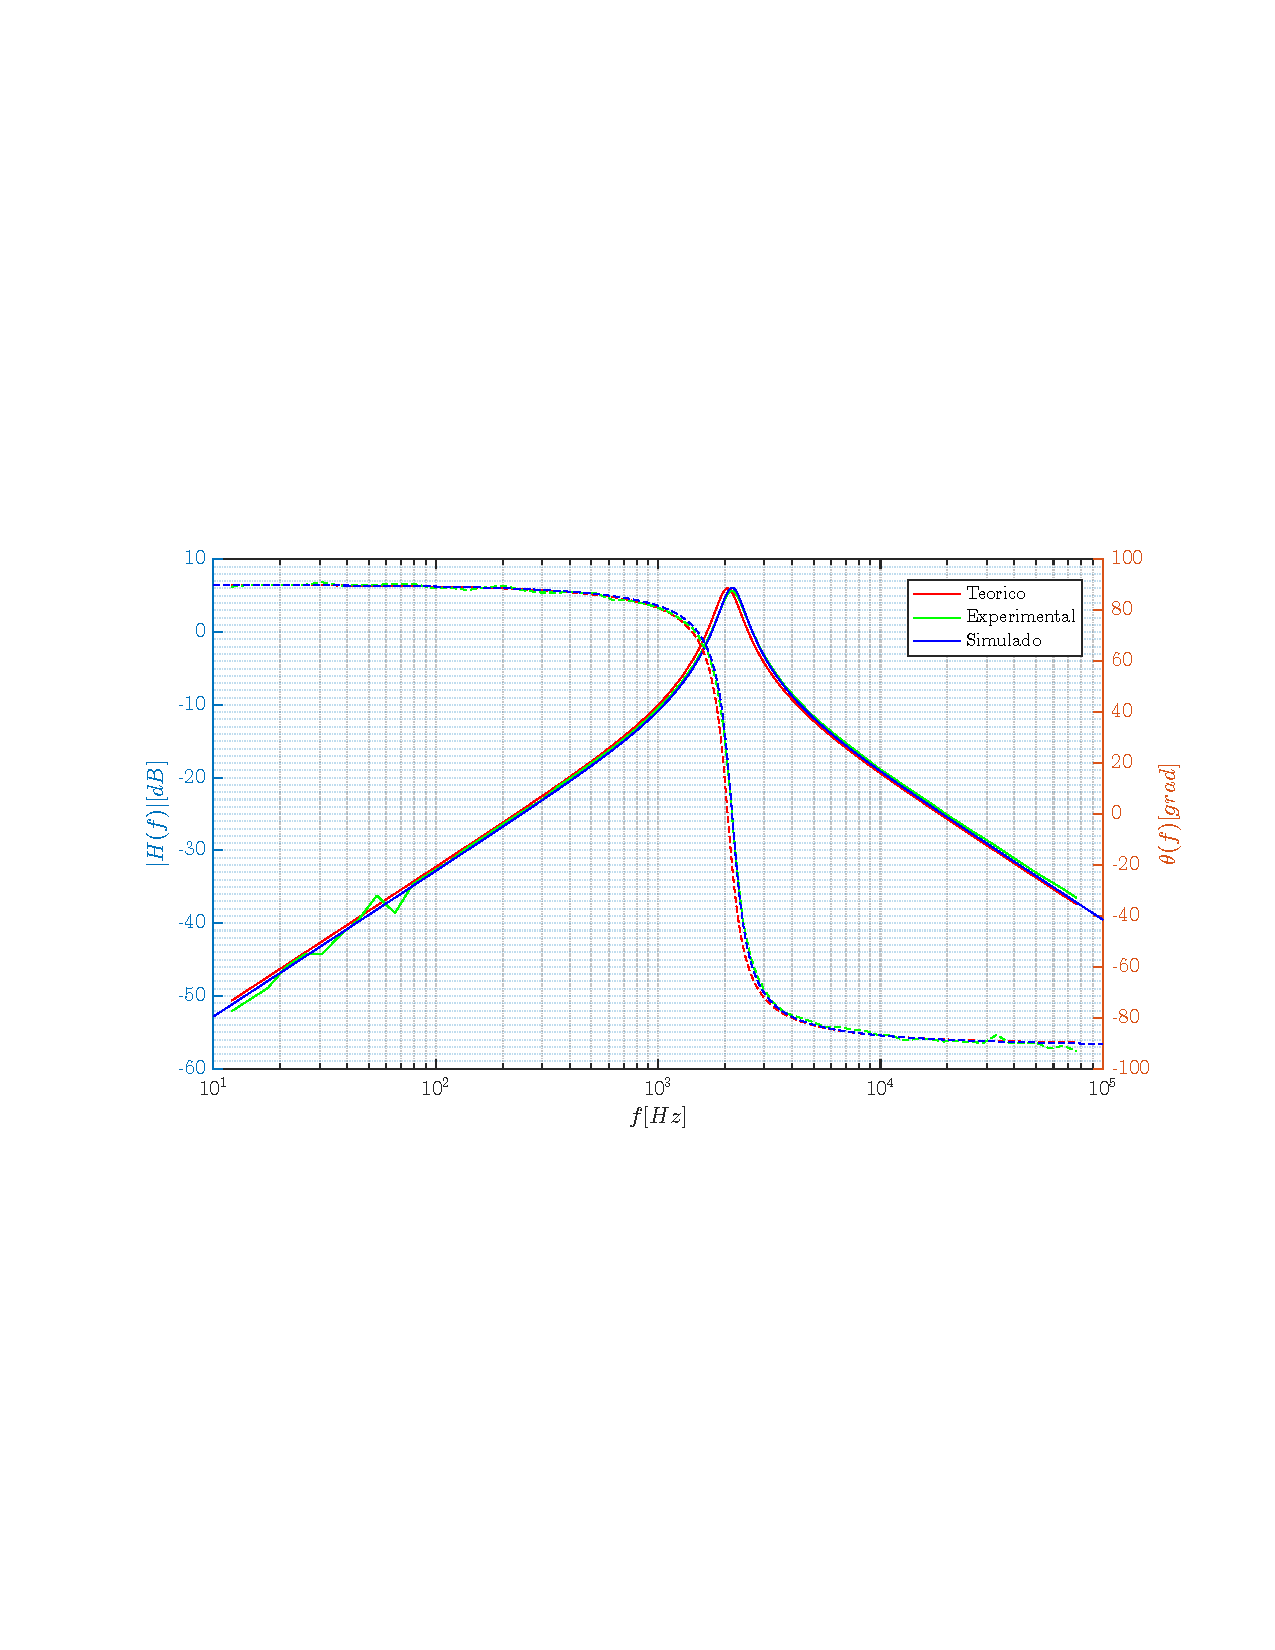
\includegraphics[scale=0.4]{resources/bode_todos}
\caption{Diseño final del circuito impreso}
\label{1_bode}
\end{figure}

\subsubsection{Impedancia de entrada}
Las figuras muestran la magnitud y la fase de la impedancia de entrada medida sobre el circuito implementado contra las calculadas. La impedancia de entrada calculada se muestra en la Expresión

\begin{figure}[H]
\centering
\includegraphics[scale=0.4]{resources/impedancia_entrada_mag}
\caption{Magnitud de impedancia de entrada medida vs. calculada}
\label{1_zin_mag}
\end{figure}

\begin{figure}[H]
\centering
\includegraphics[scale=0.4]{resources/impedancia_entrada_phase}
\caption{Fase de impedancia de entrada medida vs. calculada}
\label{1_zin_phase}
\end{figure}

\begin{equation}
Z_{in}(\$) = \frac{R_6R^2C^2\$^2 + R^2C\$ + R6}{R^2C^2\$^2 + 1}
\label{1_zin_teo}
\end{equation}

\subsubsection{Error}

Las figuras \ref{1_mc_mag} y \ref{1_mc_phase} muestran los resultados obtenidos del análisis de Montecarlo realizado mediante la herramienta de simulación LTSpice. Para lograr observar las dispersiones se recortó el rango de frecuencias graficado entre 1kHz y 10kHz.

\begin{figure}[H]
\centering
\includegraphics[scale=0.4]{resources/montecarlo_mag}
\caption{Análisis de Montecarlo. Transferencia en magnitud del circuito}
\label{1_mc_mag}
\end{figure}

\begin{figure}[H]
\centering
\includegraphics[scale=0.4]{resources/montecarlo_phase}
\caption{Análisis de Montecarlo. Transferencia de fase del circuito}
\label{1_mc_phase}
\end{figure}

El análisis se realizo imponiendo una tolerancia para los resistores del $5\%$ y del $10\%$ para los capacitores. En base a los datos arrojados por la simulación se realizó un cálculo de errores sobre la frecuencia central $f_0$. El máximo error absoluto calculado fue de $148.86Hz$, que representa un error porcentual del $7.25\%$


\section{Respuesta al escalón}
Se midió la respuesta al escalón del sistema, obteniéndose los resultados mostrados en la Figura \ref{1_step_response}. Las curvas correspondientes a la respuesta simulada y la respuesta teórica calculada se encuentran superpuestas, de forma tal que se dificulta observar la ínfima diferencia entre las curvas. Por otro lado, la curva de la respuesta al escalón medida, presenta una leve diferencia respecto a la respuesta teórica, aunque la misma se ajusta a la respuesta esperada.

\begin{figure}[H]
\centering
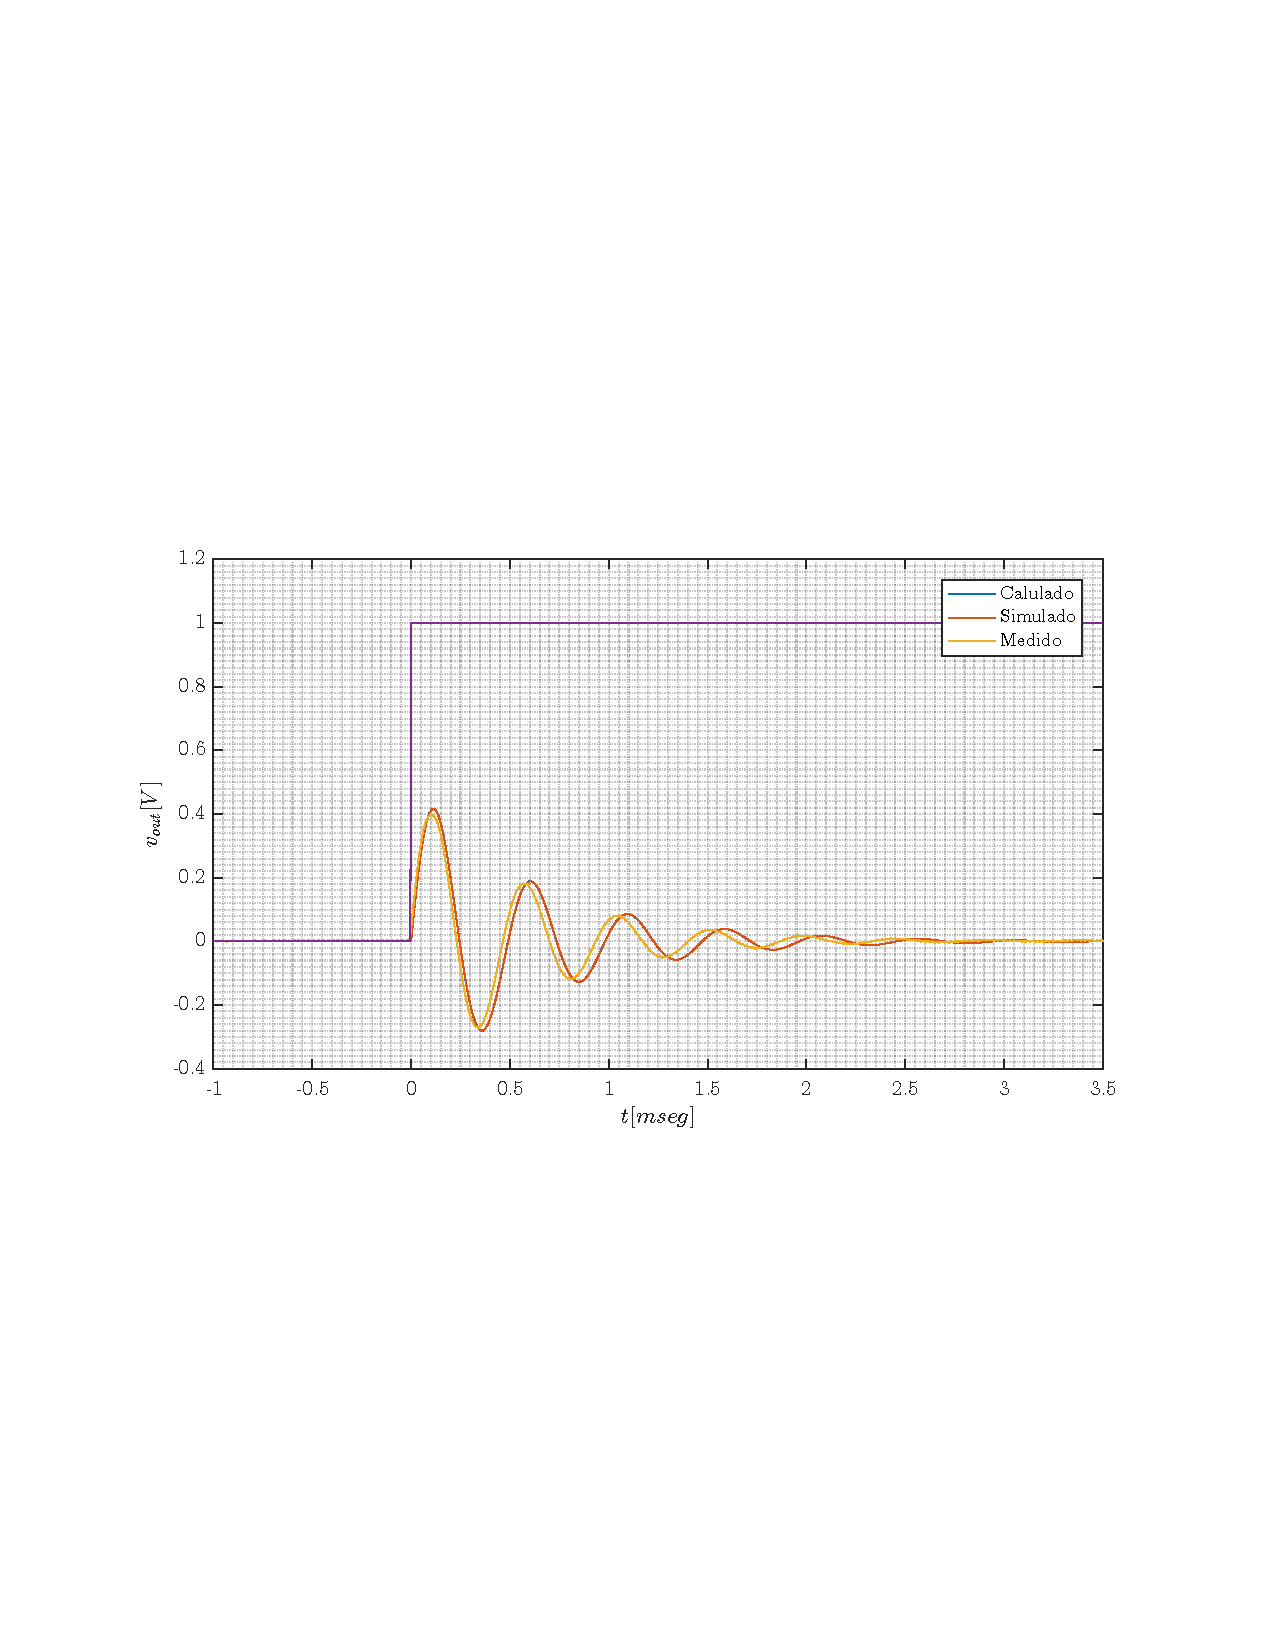
\includegraphics[scale=0.4]{resources/step_response}
\caption{Respuesta al escalón calculada, simulada y medida}
\label{1_step_response}
\end{figure}

La respuesta observada evidencia un sistema sub-amortiguado. Esto ya había quedado en evidencia en la caracterización de los polos de la transferencia del circuito, en la sección \ref{1_seccion_r6}

\section{Conclusiones}
Del análisis realizado sobre el circuito presentado en el desarrollo del informe, se pueden concluir dos ítem destacables. En primer lugar se destaca la precisión con la que los datos exprerimentales se ajustan a los cálculos realizados.
Por otro lado, y como principal objeto del informe, se debe destacar la buena aproximación a una inductancia 'real' que proporciona el circuito GIC. 

%Punto 2
\pagebreak
\documentclass[12pt,a4paper]{article}
\usepackage[utf8]{inputenc}
\usepackage[siunitx,american]{circuitikz}
\usepackage{pgfplots}
\usepackage[margin=0.5in]{geometry}
\usepackage{textcomp}
\usepackage[spanish, es-tabla]{babel}
\usepackage{amsmath}
\usepackage{graphicx}
\usepackage[colorinlistoftodos]{todonotes}
\usepackage{amsmath}
\usepackage{tikz}
\usepackage{booktabs}
\usetikzlibrary{arrows}


\usepackage{parskip}
\usepackage{fancyhdr}
\usepackage{vmargin}
\setmarginsrb{3 cm}{2.5 cm}{3 cm}{2.5 cm}{1 cm}{1.5 cm}{1 cm}{1.5 cm}


\pgfplotsset{compat=1.15}

\begin{document}

\part{Introducción al diseño de filtros activos}
\section{Introducción teórica del \textit{Gyrator}}
El concepto de \textit{Gyrator} fue introducido en 1948 por Bernard D.H.Tellegen como el hipotético quinto elemento linear luego del capacitor, inductor, resistencia y
el transformador ideal. Es un elemento electrónico de dos puertas no reciproco cuyo símbolo se puede ver en la Figura \ref{ej2_gyrator_symbol}.

\begin{figure}[h!]                                                       
    \centering\includegraphics[width=0.4\textwidth, height=4cm]{Resources/ej2_gyrator_symbol.png}
    \caption{Símbolo del \textit{Gyrator}}
    \label{ej2_gyrator_symbol}
    \end{figure}

El coeficiente $G$ tiene dimensiones de $\frac{1}{\Omega}$ y por ello se le da el nombre de \textit{Gyrator conductance}. Luego, su inversa $\frac{1}{G} = R$ se define como \textit{Gyrator resistance}. Esta resistencia tiene una direccion asociada que 
se indica por una flecha, como se puede apreciar en la Figura \ref{ej2_gyrator_symbol}. Invertir el sentido de la flecha es negar la resistencia del \textit{Gyrator} o que es lo mismo que invertir
la polaridad del puerto. A continuación se definen las ecuaciones del \textit{Gyrator} , que se depreden de la figura anteriormente mencionada:

\begin{equation} I_{1} = G V_2 \label{ej2_ecua_gyrator_1}\end{equation}
\begin{equation} I_{2} =  -G V_1 \label{ej2_ecua_gyrator_2}\end{equation}


Gracias (\ref{ej2_ecua_gyrator_1}) y (\ref{ej2_ecua_gyrator_2}) se pueden enumerar las siguientes propiedades de un \textit{Gyrator} ideal:    

\begin{enumerate}
	\item Potencia instantánea nula \\
        \begin{displaymath} P = V_1 I_1 + V_2 I_2 \end{displaymath}
        \begin{displaymath} P = (-G I_2)I_1 + (G I_1) I_2 \end{displaymath}
        \begin{displaymath} P = 0 \end{displaymath}
    
	\item Parámetros de impedancia $Z$ y parámetros de admitancia $Y$ \\
        %poner las matrices Z y Y. Es necesario ?????
	\item Inversión de impedancia de elementos lineales\\
        Si se conecta una impedancia $Z_2$ en las terminales de salida del \textit{Gyrator} y $Z_1$ es la impedancia en las terminales de entrada, se deduce lo siguiente:
        \begin{displaymath} Z_2 = \frac{V_2}{-I_2} \end{displaymath}
        \begin{displaymath} \frac{V_2}{-I_2} = \frac{\frac{-I_1}{G}}{ -G V_1} \end{displaymath}
        \begin{displaymath} \frac{V_2}{I_2} = \frac{I_1}{G^2 V_1} \end{displaymath}
        \begin{displaymath} Z_2 = \frac{1}{Z_1 G^2} \end{displaymath}
        \begin{displaymath} Z_1 = \frac{1}{Z_2 G^2} \end{displaymath}

        Esto implica que si se conecta, por ejemplo, una resistencia lineal $R_L$ en las terminales de salida del \textit{Gyrator}, la entrada se comporta como
        una resistencia lineal de impedancia $ \frac{1}{R_L G^2} $. Luego, se puede lograr que una capacidad se comporte como una inductancia. Esta propiedad es sumamente interesante
        ya que se puede utilizar al \textit{Gyrator} para realizar filtros sin inductores. Antes del desarrollo del transistor, los inductores eran grandes y costosos por lo que su uso traían varios problemas. Gracias al \textit{Gyrator}
        se puede sustituir al inductor y sobrepasar este tipo de problemas. Esta propiedad es la que mas se utiliza a lo largo de toda esta sección. La Figura \ref{ej2_gyrator_prop2} muestra esta propiedad.
        Nótese que, un capacitor de valor $C$ a la salida de un \textit{Gyrator} ideal hace que a la entrada halla una inductancia igual a:

        \begin{equation} L =  \frac{C}{G^2} \label{ej2_ecua_gyrator_inversion_impedancia}\end{equation}

        \begin{figure}[h!]                                                       
            \centering\includegraphics[width=0.7\textwidth, height=4cm]{Resources/ej2_gyrator_prop2.png}
            \caption{Propiedad de inversión de impedancia}
            \label{ej2_gyrator_prop2}
            \end{figure}
    
    \item Inversión corriente - voltaje \\
        De (\ref{ej2_ecua_gyrator_1}) y (\ref{ej2_ecua_gyrator_2}) se ve claramente que si la salida de un \textit{Gyrator} ideal tiene una fuente de tensión , por ejemplo, $E$ a la entrada tendrá una fuente de corriente $I_1 = G V_2$. 
        En la Figura \ref{ej2_gyrator_prop3} se puede apreciar esta propiedad con mayor detalle.  

        \begin{figure}[h!]                                                       
            \centering\includegraphics[width=0.7\textwidth, height=4cm]{Resources/ej2_gyrator_prop3.png}
            \caption{Propiedad de inversión corriente - voltaje}
            \label{ej2_gyrator_prop3}
            \end{figure}
    

\end{enumerate}


\section{\textit{Gyrator} como inductor}

Como se vio anteriormente, las propiedades del \textit{Gyrator} hacen posible simular un inductor con un capacitor. El objetivo de esta sección es realizar un circuito que simule un inductor para poder utilizarlo en el armado de filtros activos. 
En la Figura \ref{ej2_inductor_model} se puede ver el modelo del inductor. Si se define su impedancia de entrada como $Z_{in}$:

\begin{equation} Z_{in} = R_L + sL \label{ej2_ecua_inductor}\end{equation}

\begin{figure}[h!]                                                       
    \centering\includegraphics[width=0.4\textwidth, height=4cm]{Resources/ej2_inductor_model.png}
    \caption{Modelo del inductor}
    \label{ej2_inductor_model}
    \end{figure}


\begin{figure}[h!]                                                       
    \centering\includegraphics[width=0.4\textwidth, height=4cm]{Resources/ej2_gyrator_inductor.png}
    \caption{\textit{Gyrator} equivalente a un inductor}
    \label{ej2_gyrator_inductor}
    \end{figure}



Se propone el circuito de la Figura \ref{ej2_gyrator_inductor}. Este es un \textit{Gyrator} que simula inductor. Esta compuesto por un amplificador operacional (en configuración de \textit{Buffer}), resistencias y capacitores. A continuación se calcula su impedancia de entrada para analizar 
bajo que condiciones se puede considerar al circuito como un inductor. Es decir, lograr que el circuito \ref{ej2_gyrator_inductor} se parezca al circuito \ref{ej2_inductor_model}.

Se comienza con la ecuación del amplificador operacional. Si se considera que $V_{out}$ es la tensión de salida del \textit{Buffer}
\begin{displaymath} V_{out} = A_{vol} (V^+ - V^-) \end{displaymath}
\begin{displaymath} V^- = A_{vol} (V^+ - V^-) \end{displaymath}
\begin{displaymath} V^- = V^+\frac{A_{vol}}{1+A_{vol}} \end{displaymath}  
\begin{displaymath}  si \hspace{2mm} K = \frac{A_{vol}}{1+A_{vol}} \end{displaymath} 

\begin{equation} V^- = V^+K \label{ej2_ecua_aux_1}\end{equation}


Nótese que se considera al amplificador operacional sin corrientes de bias ni tensiones de offset.

Se continua con la tensión de entrada al circuito, $V_{in}$. Por divisor de tensión, $V_{in}$ es:

\begin{equation} V^+ = V_{in} \frac{R}{R+\frac{1}{sC}} \label{ej2_ecua_aux_2}\end{equation}

Si se juntan (\ref{ej2_ecua_aux_1}) y (\ref{ej2_ecua_aux_2}):
\begin{displaymath} V^- = V_{in} \frac{R}{R+\frac{1}{sC}} K \end{displaymath}

Si se define $I_1$ como la corriente que circula por $R_L$:

\begin{displaymath} I_1 = \frac{V_{in} - V^-}{R_L} \end{displaymath}

\begin{displaymath} I_1 = \frac{V_{in}}{R_L}[1-\frac{R_1}{R_1 + \frac{1}{sC}}K] \end{displaymath}

Si se define $I_2$ como la corriente que circula por $R$ y $C$:    

\begin{displaymath} I_2 = \frac{V_{in} - 0}{R + \frac{1}{sC}} \end{displaymath}

Si se define $I_{in}$ como la corriente entrante al circuito:
\begin{displaymath} I_{in} = I_1 + I_2 \end{displaymath}
\begin{displaymath} I_{in} = \frac{V_{in}}{R_L}[1-\frac{R_1}{R_1 + \frac{1}{sC}}K]  + \frac{V_{in}}{R + \frac{1}{sC}}  \end{displaymath}
\begin{displaymath} I_{in} = V_{in}[\frac{R + \frac{1}{sC} - RK + R_L}{R_L (R + \frac{1}{sC})}]  \end{displaymath}
\begin{displaymath} Z_{in} = \frac{V_{in}}{I_{in}} = \frac{R_L (R + \frac{1}{sC})}{R + \frac{1}{sC} - RK + R_L }  \end{displaymath}

\begin{equation} Z_{in} = \frac{sC R_L R + R_L}{sCR - RsCK +sCR_L + 1} \label{ej2_ecua_impedancia_entrada}\end{equation}

Al tener la expresión de la impedancia de entrada del circuito en la ecuación (\ref{ej2_ecua_impedancia_entrada}) es posible definir condiciones para lograr que se parezca a la ecuación (\ref{ej2_ecua_inductor}).
Para lograrlo se vuelve a la ecuación (\ref{ej2_ecua_aux_1}). Si se considera el modelo del polo dominante, $K$ sufre modificaciones:

\begin{displaymath} V^- = V^+ K = V^+\frac{A_{vol}}{1+A_{vol}} \end{displaymath}  
\begin{displaymath} V^- = V^+\frac{[\frac{A_{0}}{1+\frac{s}{\omega_P}}]}{1+[\frac{A_{0}}{1+\frac{s}{\omega_P}}]} \end{displaymath}  
\begin{displaymath} V^- = V^+ \frac{A_0}{1+ \frac{s}{\omega_P} + A_0} \end{displaymath}  
\begin{displaymath} V^- = V^+ \frac{A_0}{[1+ A_0]} \frac{1}{1+ \frac{s}{\omega_P [1 + A_0]}} \end{displaymath}  
\begin{displaymath} si \hspace{1mm} A_0 + 1 \simeq A_0 \end{displaymath}  
\begin{displaymath} V^- = V^+ \frac{1}{1 + \frac{s}{A_0 \omega_P}}  \end{displaymath}  
\begin{displaymath} A_0 \omega_P = BWP \hspace{1mm}(Band\hspace{1mm}Width\hspace{1mm}Product) \end{displaymath}  
\begin{displaymath} V^- = V^+ \frac{1}{1 + \frac{s}{BWP}}  \end{displaymath}  
Luego, el nuevo $K$ es:
\begin{displaymath} K = \frac{1}{1 + \frac{s}{BWP}}  \end{displaymath}  
Como se puede observar, $K$ es asemeja a la trasferencia de un pasabajos con frecuencia de corte en $f_c = \frac{BWP}{2\pi}$. Luego, si se trabaja en frecuencias menores a $f_c$ se puede tomar $K=1$. Como criterio se toma que esta frecuencia de trabajo $f$ sea 
a lo sumo igual a la frecuencia una decada antes de $f_c$. Entonces:

\begin{equation} f < \frac{BWP}{10 *2\pi} \label{ej2_ecua_condicion_1}\end{equation}

Nótese que, como $BWP$ es del orden de los $MHz$, $K$ comienza a obtener importancia cuando se trabaja en frecuencias del orden de los $MHz$. Consecuentemente, cuando se trabaje en este orden de frecuencias, se debe considerar el efecto del polo dominante.  


Volviendo a (\ref{ej2_ecua_impedancia_entrada}), si se impone el nuevo $K$ la ecuación queda:
\begin{displaymath} Z_{in} = \frac{sC R_L R + R_L}{sCR_L + 1} \end{displaymath}  
\begin{equation} Z_{in} = \frac{R_L [sCR + 1]}{sCR_L + 1} \label{equ:ej2_impedancia_gyrator} \end{equation}  
    
Algo muy interesante para observar es que, al imponer que $K=1$ es indistinto si se conecta el buffer a la entrada inversora o a la entrada no inversora. 


Al tener la expresión de la impedancia de entrada (\ref{equ:ej2_impedancia_gyrator}) se puede ver que la misma cuenta con un cero en $\frac{1}{CR}$ y un polo en $\frac{1}{R_L C}$. Para una mayor comprensión, se simula el circuito del \textit{Gyrator}. En la Figura \ref{ej2_sim_inductor} se puede ver una simulación dándole los siguientes valores a los componentes: 

\begin{table}[h!]
    \centering
    \begin{tabular}{@{}cc@{}}
    \toprule
    Componente   & Valor \\ \midrule
    \text{C}   & 100nF \\
    \text{$R$}   & $1k\Omega$     \\
    \text{$R_L$} & $10\Omega$    \\ 

    \end{tabular}
    \caption{Componentes del \textit{Gyrator}}
    \label{ej2_sim_inductor}
    \end{table}
    

\begin{figure}[h!]                                                       
    \centering\includegraphics[width=0.9\textwidth, height=9cm]{Resources/ej2_gyrator_sim.png}
    \caption{Simulación de \textit{Gyrator} }
    \label{ej2_sim_inductor}
    \end{figure}

Esta ultima figura muestra el comportamiento de un pasa banda. Sin embargo, la parte de interés es cuando se comporta como una bobina. Esta zona de interés es justamente antes de que el polo entre en acción. Habiendo dicho esto, lo ideal seria que el polo (osea el denominador)
de la impedancia no existiera. Si se cumple esta condición, la impedancia seria idéntica al modelo del inductor (\ref{ej2_ecua_inductor}). Luego para que el denominador sea igual a 1, se debe cumplir que $scR_L << 1 $. 

Se impone una nueva condición:

\begin{displaymath} sCR_L << 1 \end{displaymath}  
\begin{displaymath} sCR_L < 1 * 0,05 \end{displaymath}  
\begin{displaymath} f 2\pi CR_L < 1 * 0,05 \end{displaymath} 
\begin{equation} f < \frac{0.1}{2 \pi R_L C} \label{ej2_ecua_condicion_2} \end{equation}

Esta ultima condición implica que el termino $sCR_L$ debe ser despreciable frente a la unidad para todo el rango de frecuencias en que se desea que el \textit{Gyrator} funcione como (\ref{ej2_ecua_inductor}). Entonces, se puede imponer como regla que $R_L$ debe ser de valor chico (del orden de los $\Omega$) y que $C$ debe ser de valor de, por ejemplo, del orden de los nano Faradios. Como se vera mas adelante, si se utiliza $C = 100n$ y $R_L = 10\Omega$, se pude obtener un rango de trabajo considerable. 

Todas las ecuaciones obtenidas son validas siempre y cuando se cumplan las condiciones anteriormente mencionadas (\ref{ej2_ecua_condicion_1}) y (\ref{ej2_ecua_condicion_2}). Ademas, se debe tener en cuenta que se hizo todo el análisis considerando que el \textit{Gyrator} este conectado a tierra por lo que esta es una nueva condición para tener en cuenta. 

Para concluir se puede hacer una síntesis de los valores hallados:

Si se trabaja a una frecuencia menor a $f = \frac{BWP}{10 *2\pi}$ y el termino $sCR_L$ se mantiene despreciable frente a la unidad, la impedancia del \textit{Gyrator} es:

\begin{displaymath} Z_{in} = R_L + sC R_L R \end{displaymath}

Donde, 

\begin{equation} L = C R_L R \label{ej2_ecua_gyrator_3}\end{equation}
%\begin{equation} R = R_{\textit{Gyrator}} = \frac{L}{C R_L} \label{ej2_ecua_gyrator_4}\end{equation}    
%\begin{equation} |Z_{in}| = \sqrt{(2\pi CR_LR)^2 + R_L^2} \label{ej2_ecua_gyrator_4}\end{equation}
%\begin{equation} Z_{in} = \arctan(2\pi CR)\label{ej2_ecua_gyrator_4}\end{equation}    




\section {Diseño de filtros activos con \textit{Gyrator}}
En esta sección se analizan y diseñan cuatro filtros activos de segundo orden con \textit{Gyrators}. En todos los filtros se considera que el amplificador operacional tiene $r_d = \infty$ y $r_0 = 0$. Ademas, se considera que el amplificador no tiene
ni corrientes de bias ni tensiones de offset.  


\subsection{Filtro pasa altos}
El objetivo de esta sección es diseñar un filtro pasa altos que involucre el uso de un \textit{Gyrator}. El mismo debe cumplir cierta plantilla por lo que se debe estudiar la función transferencia y analizar principalmente el comportamiento del \textit{Gyrator}. 


\subsubsection{Plantilla}
La plantilla para el filtro pasa altos es la siguiente:

\begin{enumerate}
	\item Ganancia unitaria cuando $f \rightarrow \infty$
	\item Ganancia mayor a $-3dB$ para $f>f_p = 14k$
	\item Ganancia menor a $-10dB$ para $f<f_a = 4k$
	\item Ganancia nunca superior a $0dB$  
\end{enumerate}

Haciendo un análisis previo de estas condiciones, se puede decir que que la mas critica es la condición numero 4. Esta condición impone que el filtro no tenga ningún sobrepico por lo que se deben tener ciertas precauciones. Dichas precauciones se debaten mas adelante. En cuanto a la condición 1, la misma exhibe gran complejidad. Como se vio en la sección de estudio del \textit{Gyrator}, el mismo tiene un rango de frecuencias para la cual se comporta como un inductor. Entonces, se puede decir de ante mano que para cierta frecuencia (cuando el \textit{Gyrator} deje de ser un inductor) el circuito pase a comportarse de manera indeseada y no se podrá cumplir la condición 1. Todo esto quedara mas claro al avanzar en el diseño del filtro. 

\subsubsection{Funcion transferencia y circuito de segundo orden}

Un circuito clásico de segundo orden que representa un pasa altos es un RCL con salida en la inductancia. En la Figura \ref{ej2_filto_HP} se puede ver dicho circuito. 
%Grafico clasico RCL
\begin{figure}[h!]                                                       
    \centering\includegraphics[width=5cm, height=3cm]{Resources/ej2_hp.png}
    \caption{Pasa altos de segundo orden}
    \label{ej2_filto_HP}
    \end{figure}


La función transferencia de este circuito es:

\begin{displaymath} H(j\omega)= H_{0HP} H_{HP} \end{displaymath}  
Donde $H_{0HP}$ es la ganancia en altas frecuencias. Por la condición 1, $H_{0HP} = 1$. Luego:   

\begin{equation} H(j\omega) = \frac{-(\frac{\omega}{\omega_0})^{2}}{1 - (\frac{\omega}{\omega_0})^{2} + (\frac{j\omega}{\omega_0})\frac{1}{Q}} \label{equ:trans_clasica_hp}\end{equation}  

Donde $Q$ es el factor de calidad y $\omega_0$ es la frecuencia de corte.      
Al tener conocimiento de la función transferencia $H(jw)$ es posible proponer un circuito para tratar de obtener una nueva función transferencia que se asemeje lo mas posible a $H(jw)$. 

\subsubsection{Circuito propuesto}
Teniendo en mente el circuito de la Figura \ref{ej2_filto_HP}, se propone un nuevo circuito reemplazando el inductor por un \textit{Gyrator}. El circuito resultante se muestra en la Figura \ref{fig:ej2_HP_propuesto}. 

%Circuito propuesto
\begin{figure}[!]                                                       
    \centering\includegraphics[width=0.4\textwidth, height=4cm]{Resources/ej2_hp_gyrator.png}
    \caption{Circuito propuesto}
    \label{fig:ej2_HP_propuesto}
    \end{figure}

Nótese que la impedancia del \textit{Gyrator} es $Z = R_L + sR_L R C$ (si se cumple (\ref{ej2_ecua_condicion_2})) como se vio en la sección anterior. El circuito propuesto tiene la siguiente función transferencia:

\begin{displaymath} H(s)= \frac{V_{out}}{V_{in}} = \frac{R_L + sL}{(R_1 + R_L) +sL + \frac{1}{sC_1}} \end{displaymath}  
\begin{displaymath} H(s)= \frac{[R_L + sL]sC_1}{[R_1 + R_L]sC_1 +s^2LC_1 + 1} \end{displaymath}
\begin{displaymath} H(s)= \frac{s^2CR_LRC_1 + sC_1R_L}{s^2[CR_LRC_1] + s[R_1 + R_L]C_1 + 1} \end{displaymath}

Donde:

\begin{displaymath} \omega_0^2= \frac{1}{CR_LRC_1} \end{displaymath}  
\begin{displaymath} \frac{1}{\omega_0 Q}= (R_1 + R_L) C_1 \end{displaymath}  


Estas expresiones permiten proseguir en la selección de componentes. 


\subsubsection{Diseño del circuito}

Según la plantilla de este filtro, la frecuencia de corte se ubica en $f = 14kHz$. Entonces, $w_0 = 2\pi 14$. Ademas, la plantilla prohíbe tener una ganancia mayor a $0 dB$ para cualquier frecuencia. Esto implica que no pude haber un sobre pico para ninguna frecuencia. Luego, como el parámetro $Q$ es el responsable de que halla sobrepicos en este tipo de filtros, se define  $Q=\frac{1}{\sqrt{2}}$. Dicho valor de $Q$ es el mas grande que puede adquirir antes de que halla sobrepico. Entonces, se asegura que la ganancia nunca supere los $0dB$.  


Ademas se imponen se impone que $R_L = 10 \Omega$ y que $ C = 100nF$ ya que de esta manera se obtiene un buen rango para el cual el \textit{Gyrator} funciona como inductor (se cumple la condición \ref{ej2_ecua_gyrator_2}). Este tema se analiza con mas profundidad en la sección \textit{Simulación y análisis}.

Por ultimo, se define $C_1 = C$ por el simple hecho que simplifica notablemente las expresiones. 

Gracias a todas estas definiciones se pueden obtener dos expresiones para $R$ y $R_1$ y sus valores.  

Luego:

\begin{displaymath} R = \frac{1}{C^2 R_L \omega_0^2} = 1292.36 \Omega \end{displaymath}  
\begin{displaymath} R_1 = \frac{1}{\omega_0 Q C} - 10 = 150.77 \Omega \end{displaymath}  

Si $R$ y $R_1$ adquieren estos valores, se cumplen las condiciones de la plantilla. 

También es de particular interés ver como es afectada la función transferencia bajo estas definiciones:

\begin{displaymath} H(s)= \frac{s^2 10 C ^2 R + sC10}{s^2[C^2 10 R] + s[R_1 + 10]C + 1} \end{displaymath}

Nótese a primera vista la función trasferencia no es exactamente igual a la función transferencia del pasa altos clásica (\ref{equ:trans_clasica_hp}). Sin embargo, si se evaluá a la función con los valores definidos, el termino $sC10$ del numerador es $j2\pi * 1\mathrm{e}{-17}$. Este termino es prácticamente despreciable frente a $s^2 10 C^2 R_L$  por lo que la función trasferencia resulta ser:


\begin{displaymath} H(s)= \frac{s^2 1.5\mathrm{e}{-10}}{s^2[1.5\mathrm{e}{-10}] + s[1.6\mathrm{e}{-5}] + 1} \end{displaymath}


Como no existen los valores comerciales de resistencias $1292.36 \Omega$ y $150.77 \Omega$, estos se redondean para poder realizar el circuito. En la Tabla  \ref{tab:hp_components} se enumeran los componentes utilizados. 

\begin{table}[h!]
    \centering
    \begin{tabular}{@{}cc@{}}
    \toprule
    Componente   & Valor \\ \midrule
    \text{C}   & 100nF \\
    \text{$C_1$}   & 100nF \\
    \text{R}   & $1.5k\Omega$     \\
    \text{$R_L$} & $10\Omega$    \\ 
    \text{$R_1$} & $150\Omega$    \\ \bottomrule
    \end{tabular}
    \caption{Componentes del circuito propuesto}
    \label{tab:hp_components}
    \end{table}

Como se explico anteriormente, el objetivo es realizar cuatro filtros. Se decide, realizar los mismos en el mismo PCB y utilizando el mismo integrado. Dicho integrado es el $TL 084$ que, gracias a la \textit{datasheet} tiene un $BPW$ de $2.5MHz$. Se brinda mas información del PCB final en la sección \textit{Diseño PCB}. Al tener dicho $BPW$, y teniendo en cuenta la condición \ref{ej2_ecua_condicion_1} se debe trabajar a una frecuencia inferior a $40kHz$ para que no se consideren los efectos del polo dominante. 

Antes de continuar con la medición se realiza una simulación montecarlo para evaluar el comportamiento del circuito bajo distintos valores de componentes. Como se vera en la sección \textit{Diseño PCB}
se utilizan todos componentes de montaje superficial con tolerancias $1\%$. El resultado de la simulación se ve en la Figura \ref{fig:monte}. 

\begin{figure}[h!]                                                       
    \centering\includegraphics[width=0.9\textwidth, height=7cm]{Resources/ej2_montecarlo.png}
    \caption{Simulación de montecarlo}
    \label{fig:monte}
    \end{figure}
    
La simulación muestra una variación prácticamente imperceptible ya que las tolerancias son muy pequeñas. Se concluye que no se debe corregir los componentes. Esta simulación solo se realiza para este filtro ya que no aporta al análisis de los circuitos. 

\subsubsection{Simulacion y analisis lineal}
Si se simula el circuito propuesto (desde $f = 10 Hz$ a $f = 10MHz$) con los componentes de la Tabla \ref{tab:hf_gyrator_components}, se obtiene el gráfico de la Figura \ref{ej2_hp_sim}.

\begin{figure}[h!]                                                       
    \centering\includegraphics[width=0.9\textwidth, height=9cm]{Resources/ej2_hp_sim.png}
    \caption{Simulación del circuito propuesto }
    \label{ej2_hp_sim}
    \end{figure}

Gracias a las herramientas de LTSpice, se detecta que a la frecuencia $f = 14kHz$ hay una atenuación de $2.15 dB$. Si $f > 14kHz$ la ganancia es mayor a $-3dB$. Luego, la condición 2 se cumple. Si $f < 4kHz$, la ganancia es menor $-10dB$ por lo que la condición 3 también se cumple. Ademas, se puede ver que la ganancia nunca supera los $0dB$ por lo que la condición 4 también se cumple. 

Con respecto a la condición 1, se nota en el diagrama de bode que alrededor de $f = 195 kHz$ la atenuación deja de ser $0dB$ y comienza a aumentar. Esto se debe a que estas frecuencias el \textit{Gyrator} deja de comportarse como un inductor. Para un mejor comprendimiento e lo que sucede, se prosigue a realizar un análisis de linealidad. Gracias a este análisis se puede determinar en que frecuencias el \textit{Gyrator} adquiere la impedancia deseada (\ref{ej2_inductor_model}). Para comenzar el análisis, se simula el \textit{Gyrator} en LTSpice con los valores de $R$, $R_L$ y $C$ propuestos. El resultado se detalla en la Figura \ref{fig:ej2_HP_gyrator_sim}.

\begin{figure}[h!]                                                       
    \centering\includegraphics[width=0.9\textwidth, height=7cm]{Resources/ej2_hp_gyrator_sim.png}
    \caption{Simulación del \textit{Gyrator} }
    \label{fig:ej2_HP_gyrator_sim}
    \end{figure}

La simulación detalla como la impedancia del \textit{Gyrator} varia con la frecuencia. Nótese lo siguiente: en el rango de frecuencias que va desde $f = 14 kHz$ a $f = 100 kHz$ la impedancia adopta un comportamiento prácticamente lineal. Esto se debe a que la impedancia del \textit{Gyrator} (\ref{equ:ej2_impedancia_gyrator}) esta bajo la condición \ref{ej2_ecua_condicion_2} y se comporta como la impedancia del modelo de un inductor \ref{ej2_inductor_model}. A hasta la frecuencia de $f=100kHz$ el denominador de (\ref{equ:ej2_impedancia_gyrator}) es despreciable frente a la unidad. Al sobrepasar esta frecuencia provoca un decaimiento en la impedancia. Todo esto explica porque en la simulación del circuito propuesto (Figura \ref{ej2_hp_sim}) la atenuación aumenta a partir de la frecuencia $f = 195 kHz$. 

Cabe destacar que para ambas simulaciones se utilizo un amplificador operacional ideal. Esto hace que no se pueda apreciar los efectos del polo dominante. Los mismos se analizan en la siguiente sección al obtener la medición real del circuito. 

\subsubsection{Medicion y analisis a altas frecuencias}

Al imponer una senoide de $V_{PP} = 3V$ como señal de entrada al circuito en un rango de frecuencias de $[10Hz , 10MHz]$, se obtiene el bode de la Figura \ref{fig:ej2_hp_med_and_sim}. En dicha figura también se superpone la simulación del circuito propuesto.  

\begin{figure}[h!]                                                       
    \centering\includegraphics[width=0.9\textwidth, height=7cm]{Resources/ej2_hp_med_and_sim.png}
    \caption{Medición y simulación del circuito propuesto }
    \label{fig:ej2_hp_med_and_sim}
    \end{figure}

Se puede ver que la simulación y la medición se comportan prácticamente igual hasta aproximadamente $40kHz$. A esa frecuencia, se detecta que la medición comienza a atenuar. Esto se debe a la condición (\ref{ej2_ecua_condicion_2}). A estas frecuencias el polo dominante entra en efecto y provoca una atenuación. Esto implica que a altas frecuencias no se puede obtener una ganancia de $0dB$, como propone la plantilla. 



\subsubsection{Conclusion}

En primer lugar, se destaca que se logro hacer un filtro pasa altos sin la utilización de un inductor. Se pudo sustituir dicho componente gracias a la ayuda de la teoría de \textit{Gyrators}. También, se pudo cumplir casi con la totalidad de la plantilla propuesta. En cuanto a la condición de ganancia unitaria para frecuencias infinitas es prácticamente imposible de cumplir ya que como el \textit{Gyrator} esta compuesto de un amplificador operacional, y los amplificadores operacionales ideales no existen, siempre se tendrá el inconveniente del polo dominante. Ademas, como se vio, el \textit{Gyrator} tiene un rango de frecuencias para el cual trabaja como un inductor por lo que inevitablemente a una cierta frecuencia el circuito deja de comportarse como se desea. Se puede concluir que el rango de frecuencias de trabajo de este filtro es hasta $40kHz$. 


\subsection{Pasa Banda}

EL objetivo de esta sección es diseñar un filtro pasa bandas que, como en el caso del pasa altos, involucre el uso de un \textit{Gyrator}. El filtro también debe cumplir cierta plantilla.

\subsubsection{Plantilla}

\begin{enumerate}
	\item Frecuencia de pasabanda de $f = 8kHz$	
\end{enumerate}

Como se puede observar las condiciones de la platilla son muy flexibles ya que no se especifica las frecuencias laterales no la atenuación que estas deben tener. Se prosigue como en el caso anterior. 

\subsubsection{Funcion transferencia y circuito de segundo orden}

Un circuito clásico de segundo orden que representa un pasa bandas es un RCL con el capacitor en paralelo con la bobbina . En la Figura \ref{ej2_filto_BP} se puede ver dicho circuito. 

%Grafico clasico RCL
\begin{figure}[h!]                                                       
    \centering\includegraphics[width=5cm, height=3cm]{Resources/ej2_bp.png}
    \caption{Pasa banda}
    \label{ej2_filto_BP}
    \end{figure}


La función transferencia de este circuito es:


\begin{equation} H(j\omega) = \frac{(\frac{j\omega}{Q\omega_0})}{1 - (\frac{\omega}{\omega_0})^{2} + (\frac{j\omega}{\omega_0})\frac{1}{Q}} \label{equ:trans_clasica_bp}\end{equation}  

Donde $Q$ es el factor de calidad y $\omega_0$ es la frecuencia de corte.      
Al tener conocimiento de la función transferencia $H(jw)$ es posible proponer un circuito para tratar de obtener una nueva función transferencia que se asemeje lo mas posible a $H(jw)$. 

\subsubsection{Circuito propuesto}
Se propone el circuito de la Figura \ref{fig:ej2_BP_propuesto}. 

%Circuito propuesto
\begin{figure}[!]                                                       
    \centering\includegraphics[width=0.4\textwidth, height=4cm]{Resources/ej2_bp_gyrator.png}
    \caption{Circuito propuesto}
    \label{fig:ej2_BP_propuesto}
    \end{figure}

Se puede extraer la siguiente función transferencia:

\begin{displaymath} H(s)= \frac{V_{out}}{V_{in}} = \frac{R_L + sL}{[1+sC R_L + s^2 C L] [R_1 + \frac{R_L + sL}{1 + sCR_L + s^2 C L}]} \end{displaymath}  
\begin{displaymath} H(s)= \frac{\frac{R_L + sL}{[R_1 + R_L]}}{\frac{s^2 C_1 L R_1}{[R_1 + R_L]} + \frac{s C_1 R_L R_1 + L}{R_1 + R_L} +1} \end{displaymath}
\begin{displaymath} H(s)= \frac{\frac{R_L + sCR R_L}{[R_1 + R_L]}}{\frac{s^2 C_1 CR R_L R_1}{[R_1 + R_L]} + \frac{s C_1 R_L R_1 + CR R_L}{R_1 + R_L} +1} \end{displaymath}

Donde:

\begin{displaymath} \omega_0^2= \frac{R_1 + R_L}{CR_LRC_1 R_1} \end{displaymath}  
\begin{displaymath} \frac{1}{\omega_0 Q}= \frac{C_1 R_L R_1 + R_L R C}{R_1 + R_L} \end{displaymath}  





\subsubsection{Diseño del circuito}


Al igual que en el filtro anterior, se seleccionan los componentes. Como se obtuvieron en el filtro anterior muy buenos resultados al definir $R_L = 10 \Omega$ y $ C = 100nF$, se utilizan los mismos valores. En este caso se define $Q = 1$,  $C_1 = C$ y $\omega_0 = 2\pi 8k$. 


Gracias a todas estas definiciones se pueden obtener dos ecuaciones que dependen tanto de  $R$ y $R_1$:.  

Luego:

\begin{displaymath} R = \frac{R_1 + R_L }{C^2 R_L R_1 \omega_0^2} = 4147.26 \Omega \end{displaymath}  
\begin{displaymath} R_1 = \frac{R_L R C - \frac{R_L}{\omega_0 Q}}{\frac{1}{\omega_0 Q} - R_L C} = 208.96 \Omega \end{displaymath} 


Al tener los valores de todos los componentes, se puede formar la Tabla  \ref{tab:bp_gyrator_components} de los componentes utilizados. 

\begin{table}[h!]
    \centering
    \begin{tabular}{@{}cc@{}}
    \toprule
    Componente   & Valor \\ \midrule
    \text{C}   & 100nF \\
    \text{$C_1$}   & 100nF \\
    \text{$R_A$}   & $3.9k\Omega$     \\
    \text{$R_B$}   & $240\Omega$     \\
    \text{$R_L$} & $10\Omega$    \\ 
    \text{$R_1$} & $200\Omega$    \\ \bottomrule
    \end{tabular}
    \caption{Componentes del circuito propuesto}
    \label{tab:bp_gyrator_components}
    \end{table}

    
    
\subsubsection{Simulacion y analisis lineal}
Si se simula el circuito propuesto (desde $f = 1 Hz$ a $f = 10MHz$) con los componentes de la Tabla \ref{tab:bp_gyrator_components}, se obtiene el gráfico de la Figura \ref{ej2_bp_sim}.

\begin{figure}[h!]                                                       
    \centering\includegraphics[width=0.9\textwidth, height=9cm]{Resources/ej2_bp_sim.png}
    \caption{Simulación del circuito propuesto }
    \label{ej2_bp_sim}
    \end{figure}

Como se puede ver en la Figura, el bode describe un pasa banda. Se detecta que a la frecuencia $f = 8kHz$ hay una atenuación de $800 mdB$, siendo esta la menor atenuación en todo el rango de frecuencias. Como la plantilla no especifica las frecuencias laterales, es de interés averiguarlas mediante el bode. Las dos frecuencias en las que se detecta una atenuación de $3 dB$ son $f_1 = 5kHz$ y $f_2 = 12.2kHz$. 


Al igual que en la sección anterior, se realiza un análisis lineal. En la Figura \ref{fig:ej2_HP_gyrator_sim} se simula el circuito del \textit{Gyrator} con los correspondientes  $R_A$, $R_B$,  $R_L$ y $C$.



\begin{figure}[h!]                                                       
    \centering\includegraphics[width=0.9\textwidth, height=7cm]{Resources/ej2_bp_gyrator_sim.png}
    \caption{Simulación del \textit{Gyrator} }
    \label{fig:ej2_BP_gyrator_sim}
    \end{figure}


En la simulación del \textit{Gyrator}, se puede apreciar que la impedancia tiene un comportamiento creciente hasta que llega a una frecuencia aproximada de $f = 62 kHz$. Al sobrepasar esta frecuencia, la impedancia decae abruptamente. Como esto recién sucede a una frecuencia mucho mayor que $f=8kHz$, se puede decir que el \textit{Gyrator} se comporta como un inductor en un rango de frecuencias considerable. 

\subsubsection{Medicion y analisis a altas frecuencias}

Al imponer una senoide de $V_{PP} = 3V$ como señal de entrada al circuito en un rango de frecuencias de $[10Hz , 1MHz]$, se obtiene el bode de la Figura \ref{fig:ej2_hp_sim_y_medicion}. En dicha imagen también se superpone la simulación anteriormente mostrada para poder comparar resultados. A primera vista el resultado es muy bueno. Tanto para bajas, medias y altas frecuencias el circuito propuesto se comporta como en la simulación. Al igual que en la simulación, la frecuencia máxima se da en aproximadamente la misma frecuencia. Otra cosa para notar es el polo dominante. En este caso, el filtro se beneficia de el ya que a frecuencias altas tiende a atenuar las señales. Esto implica que la condición (\ref{ej2_ecua_condicion_1}) se puede dejar de lado.  

\begin{figure}[h!]                                                       
    \centering\includegraphics[width=0.9\textwidth, height=9cm]{Resources/ej2_bp_med_and_sim.png}
    \caption{Bode de medición y simulación}
    \label{fig:ej2_hp_sim_y_medicion}
    \end{figure}

\subsubsection{Conclusion}

Se logro utilizar un \textit{Gyrator} para crear un filtro pasa banda. Como la plantilla para este filtro es sencilla y flexible se logro crear el filtro sin mayor inconvenientes. El circuito propuesto resulto como se esperaba. La medición y la simulación se asemejan. Ambas, se comportan prácticamente igual en todo el rango de frecuencias e incluso se utiliza el factor del polo dominante a favor. Finalmente, se puede decir que este filtro funciona para un amplio rango de frecuencias que va desde bajas frecuencias ($10Hz$) hasta $10Mhz$. 







%La funcion trasferencia resulta:
%\begin{displaymath} H(s)= \frac{V_{out}}{V_{in}} = \frac{R_L + sL}{(R_1 + R_L) +sL + \frac{1}{sC_1}} \end{displaymath}  
%\begin{displaymath} H(s)= \frac{[R_L + sL]sC_1}{[R_1 + R_L]sC_1 +s^2LC_1 + 1} \end{displaymath}
%\begin{displaymath} H(s)= \frac{s^2CR_LRC_1 + sC_1R_L}{s^2[CR_LRC_1] + s[R_1 + R_L]C_1 + 1} \end{displaymath}
%Si se impone la siguiente condicion para simplificar las cuentas:
%\begin{displaymath} R_L = R \end{displaymath}
%\begin{displaymath} C_1 = C \end{displaymath}
%\begin{displaymath} H(s)= \frac{s^2 [CR_L]^2 + sCR_L}{s^2[CR_L]^2 + s[R_1 + R_L]C + 1} \end{displaymath}
%Si bien la funcion trasferencia no es exactamente igual a la funcion trasferencia clasica de un pasa altos de segundo orden, la funcion hallada sigue 
%siendo un filtro de segundo orden. 

%De la funcion trasferencia se puede obtener la frecuencia de corte $\omega_0$:

%\begin{displaymath} \omega_0 = \frac{1}{C R_L}  \end{displaymath}

%Ademas, se puede obtener una expresion para $Q$: 
%\begin{displaymath} \frac{1}{\omega_0 Q} = C_1 [R_1 + R_L]  \end{displaymath}
%\begin{displaymath} \frac{1}{\omega_0 Q} = [\frac{R_1}{R_L} + 1]  \end{displaymath}

%La condición 4 impide que halla un sobre pico. Luego, $Q$ debe tener un valor menor a $1$. Como el $Q$ mas grande antes del sobre pico es $Q=\frac{1}{\sqrt{2}}$. Entonces:
%\begin{displaymath} \frac{1}{\sqrt{2}} < C_1 [\frac{R_1}{R_L} + 1]   \end{displaymath}
%\begin{displaymath} -1 + \sqrt{2} < \frac{R_1}{R_L}  \end{displaymath}



\subsection{Rechaza banda}

En este caso se utiliza un \textit{Gyrator} para crear un filtro rechaza banda. 

\subsubsection{Plantilla}

\begin{enumerate}
\item Frecuencia donde se ubica el\textit{notch} $f = 4kHz$	
\end{enumerate}

Al igual que el pasa banda, la plantilla es muy flexible. Se prosigue a diseñar el circuito. 

\subsubsection{Funcion transferencia y circuito de segundo orden}

En la Figura \ref{ej2_filto_BR} se puede ver un circuito clásico de un filtro rechaza banda de segundo orden. 

%Grafico clasico RCL
\begin{figure}[h!]                                                       
\centering\includegraphics[width=5cm, height=3cm]{Resources/ej2_br.png}
\caption{Rechaza banda}
\label{ej2_filto_BR}
\end{figure}


La función transferencia de este circuito es:

\begin{equation} H(j\omega) = \frac{1-(\frac{j\omega}{\omega_0})^2}{1 - (\frac{\omega}{\omega_0})^{2} + (\frac{j\omega}{\omega_0})\frac{1}{Q}} \label{equ:trans_clasica_br}\end{equation}  

Donde $Q$ es el factor de calidad y $\omega_0$ es la frecuencia de corte.      
Al tener conocimiento de la función transferencia $H(jw)$ es posible proponer un circuito para tratar de obtener una nueva función transferencia que se asemeje lo mas posible a $H(jw)$. 

\subsubsection{Circuito propuesto}
Se propone el circuito de la Figura \ref{fig:ej2_BR_propuesto}. 

%Circuito propuesto
\begin{figure}[!]                                                       
\centering\includegraphics[width=0.4\textwidth, height=4cm]{Resources/ej2_br_gyrator.png}
\caption{Circuito propuesto}
\label{fig:ej2_BR_propuesto}
\end{figure}

Se puede extraer la siguiente función transferencia:

\begin{displaymath} H(s)= \frac{V_{out}}{V_{in}} = \frac{R_L + sL + \frac{1}{sC_1}}{R_L + R_1 +sL + \frac{1}{sC_1}} \end{displaymath}  
\begin{displaymath} H(s)= \frac{sC_1R_L + s^2LC_1 + 1}{s (R_L R_1)C + s^2LC_1 + 1} \end{displaymath}

\begin{displaymath} H(s)= \frac{sC_1R_L + s^2CR_LRC_1 + 1}{s (R_L R_1)C+ s^2CR_LRC_1 + 1} \end{displaymath}




Donde:

\begin{displaymath} \omega_0^2= \frac{1}{CR_LRC_1} \end{displaymath}  
\begin{displaymath} \frac{1}{\omega_0 Q}= (R_L + R_1)C \end{displaymath}  





\subsubsection{Diseño del circuito}


Al igual que en el filtro anterior, se seleccionan los componentes. Como los otros filtros, $R_L = 10 \Omega$ y $ C = 100nF$. En este caso se define $Q = \frac{1}{\sqrt{2}}$,  $C_1 = C$ y $\omega_0 = 2\pi 4k$. 


Gracias a todas estas definiciones se pueden obtener dos ecuaciones que dependen tanto de  $R$ y $R_1$.  

Luego:

\begin{displaymath} R = \frac{1}{C^2 R_L \omega_0^2} = 15831.43 \Omega \end{displaymath}  
\begin{displaymath} R_1 = \frac{1}{\omega_0 Q C} - R_L = 552.69 \Omega \end{displaymath} 


Al tener los valores de todos los componentes, se puede formar la Tabla  \ref{tab:br_gyrator_components} de los componentes utilizados. 

\begin{table}[h!]
\centering
\begin{tabular}{@{}cc@{}}
\toprule
Componente   & Valor \\ \midrule
\text{C}   & 100nF \\
\text{$C_1$}   & 100nF \\
\text{$R_A$}   & $15k\Omega$     \\
\text{$R_B$}   & $820\Omega$     \\
\text{$R_L$} & $10\Omega$    \\ 
\text{$R_1$} & $560\Omega$    \\ \bottomrule
\end{tabular}
\caption{Componentes del circuito propuesto}
\label{tab:br_gyrator_components}
\end{table}



\subsubsection{Simulacion y analisis lineal}
Si se simula el circuito propuesto (desde $f = 1 Hz$ a $f = 10MHz$) con los componentes de la Tabla \ref{tab:br_gyrator_components}, se obtiene el gráfico de la Figura \ref{ej2_br_sim}.

\begin{figure}[h!]                                                       
\centering\includegraphics[width=0.9\textwidth, height=9cm]{Resources/ej2_br_sim.png}
\caption{Simulación del circuito propuesto }
\label{ej2_br_sim}
\end{figure}

El bode claramente describe un rechaza banda. La máxima atenuación se da en $f= 4kHz$, que es a la frecuencia deseada. También, cabe destacar que la profundidad del rechaza banda es de aproximadamente $27 dB$. Se puede decir que para ser un filtro pasivo rechaza banda la profundidad obtenida es muy buena.  


Al igual que en la sección anterior, se realiza un análisis lineal. En la Figura \ref{fig:ej2_BR_gyrator_sim} se simula el circuito del \textit{Gyrator} con los correspondientes  $R_A$, $R_B$,  $R_L$ y $C$.



\begin{figure}[h!]                                                       
\centering\includegraphics[width=0.9\textwidth, height=7cm]{Resources/ej2_br_gyrator_sim.png}
\caption{Simulación del \textit{Gyrator} }
\label{fig:ej2_BR_gyrator_sim}
\end{figure}


En la simulación del \textit{Gyrator} es muy similar a las simulaciones ya realizadas. En este caso, la impedancia tiene un comportamiento creciente hasta que llega a una frecuencia aproximada de $f = 30 kHz$. Luego, la impedancia cae abruptamente. Como el pico máximo sucede a la frecuencia de $f=4kHz$, se puede decir que el \textit{Gyrator} funciona correctamente en el rango de frecuencias desde bajas frecuencias ($10Hz$) hasta $f = 30kHz$

\subsubsection{Medicion y analisis a altas frecuencias}

Se realiza un bode con una señal de entrada configurada como senoide de $V_{PP} = 3V$ desde $[10Hz , 1MHz]$. La Figura \ref{fig:ej2_hp_med_and_sim}.

\begin{figure}[h!]                                                    
\centering\includegraphics[width=0.9\textwidth, height=9cm]{Resources/ej2_br_med_and_sim.png}
\caption{Bode de medición y simulación}
\label{fig:ej2_hp_med_and_sim}
\end{figure}

Los resultados son satisfactorios. Se destaca que a bajas frecuencias y a la frecuencia del rechaza banda tanto la simulación como la medición se comportan prácticamente igual. Sin embargo, se puede ver que a la frecuencia de $20kHz$, el circuito comienza a atenuar nuevamente. Esto se asemeja con los que se dijo en el análisis lineal. Se predijo que recien $f = 30kHz$ el \textit{Gyrator} deja de funcionar como inductor por lo que, la medición, la atenuación comienza $10kHz$ antes. Este comportamiento se debe por el polo dominante. Recordar que por la condición (\ref{ej2_ecua_condicion_1}) el polo dominante comienza a afectar a $40 kHz$. Lo que sucede se debe a causa de que el \textit{Gyrator} deja de funcionar como bobina y por el polo dominante.  




\subsubsection{Conclusion}

Se cumplió el objetivo de fabricación de un filtro rechaza banda con un \textit{Gyrator}. Ademas, se logro que el filtro se adecue a la plantilla propuesta. Cabe destacar que el filtro cuenta con una profundidad muy buena. El rango de frecuencias de trabajo va desde las bajas frecuencias ($10Hz$) hasta $20kHz$. Lo ideal es que el rechaza banda funcione hasta frecuencias del orden de los $M\Omega$ pero como se vio, por causa del \textit{Gyrator} esto es imposible. 




\subsection{Pasa bajos}

Como ultimo filtro, se intenta fabricar un filtro pasa bajos con un \textit{Gyrator}.


\subsubsection{Plantilla}

\begin{enumerate}
	\item Ganancia unitaria en continua
	\item Ganancia mayor a $-3dB$ para $f<f_p = 4k$
	\item Ganancia menor a $-10dB$ para $f>f_a = 14k$
	\item Ganancia nunca superior a $0dB$
\end{enumerate}

La plantilla se asemeja mucho al filtro pasa altos. En este caso, la frecuencia de corte se situá en $f=4kHz$.

\subsubsection{Funcion transferencia y circuito de segundo orden}

En la Figura \ref{ej2_filto_LP} se puede ver un circuito clásico de un filtro pasa bajos de segundo orden. 

%Grafico clasico RCL
\begin{figure}[h!]                                                       
\centering\includegraphics[width=5cm, height=3cm]{Resources/ej2_lp.png}
\caption{Rechaza banda}
\label{ej2_filto_LP}
\end{figure}


La función transferencia de este circuito es:

\begin{equation} H(j\omega) = \frac{1}{1 - (\frac{\omega}{\omega_0})^{2} + (\frac{j\omega}{\omega_0})\frac{1}{Q}} \label{equ:trans_clasica_br}\end{equation}  

Donde $Q$ es el factor de calidad y $\omega_0$ es la frecuencia de corte.      
Al tener conocimiento de la función transferencia $H(jw)$ es posible proponer un circuito para tratar de obtener una nueva función transferencia que se asemeje lo mas posible a $H(jw)$. 

\subsubsection{Circuito propuesto}
Se propone el circuito de la Figura \ref{fig:ej2_LP_propuesto}. 

%Circuito propuesto
\begin{figure}[!]                                                       
\centering\includegraphics[width=0.4\textwidth, height=4cm]{Resources/ej2_lp_gyrator.png}
\caption{Circuito propuesto}
\label{fig:ej2_LP_propuesto}
\end{figure}


Notar que en la Figura  \ref{fig:ej2_LP_propuesto} hay dos salidas $V_{out}$ que se definen como $V_{out1}$ y $V_{out2}$. Esto se debe a  una de las condiciones del \textit{Gyrator}. Una de las condiciones del circuito propuesto del \textit{Gyrator} es que este conectado a tierra. Entonces, para mantener una consistencia con el resto de los circuitos, se debe obtener la salida de señal del capacitor. Esto se logra simplemente saliendo diferencial del capacitor, realizando $|V_{out1} - V_{out2}|$. 

Teniendo esto en cuenta, se construye la funcion transferencia:

\begin{displaymath} H(s)= \frac{V_{out}}{V_{in}} = \frac{\frac{1}{sC_1}}{R_L + R_1 +sL + \frac{1}{sC_1}} \end{displaymath}  
\begin{displaymath} H(s)= \frac{1}{s (R_L R_1)C + s^2LC_1 + 1} \end{displaymath}

\begin{displaymath} H(s)= \frac{1}{s (R_L R_1)C + s^2  C R_L R C_1 + 1} \end{displaymath}

Donde:

\begin{displaymath} \omega_0^2= \frac{1}{CR_LRC_1} \end{displaymath}  
\begin{displaymath} \frac{1}{\omega_0 Q}= (R_L + R_1)C \end{displaymath}  





\subsubsection{Diseño del circuito}


Al igual que en el filtro anterior, se seleccionan los componentes. Como los otros filtros, $R_L = 10 \Omega$ y $ C = 100nF$. En este caso se define $Q = \frac{1}{\sqrt{2}}$ ya que una de las condiciones del filtro es que nunca se sobrepase $0dB$ También, se define $C_1 = C$ y $\omega_0 = 2\pi 4k$. 


Gracias a todas estas definiciones se pueden obtener dos ecuaciones que dependen tanto de  $R$ y $R_1$.  

Luego:

\begin{displaymath} R = \frac{1}{C^2 R_L \omega_0^2} = 15831.43 \Omega \end{displaymath}  
\begin{displaymath} R_1 = \frac{1}{\omega_0 Q C} - R_L = 552.69 \Omega \end{displaymath} 


Al tener los valores de todos los componentes, se puede formar la Tabla  \ref{tab:lp_gyrator_components} de los componentes utilizados. 

\begin{table}[h!]
\centering
\begin{tabular}{@{}cc@{}}
\toprule
Componente   & Valor \\ \midrule
\text{C}   & 100nF \\
\text{$C_1$}   & 100nF \\
\text{$R$}   & $15k\Omega$     \\

\text{$R_L$} & $10\Omega$    \\ 
\text{$R_1$} & $510\Omega$    \\ \bottomrule
\end{tabular}
\caption{Componentes del circuito propuesto}
\label{tab:lp_gyrator_components}
\end{table}


\subsubsection{Simulacion y analisis lineal}
Si se simula el circuito propuesto (desde $f = 1 Hz$ a $f = 10MHz$) con los componentes de la Tabla \ref{tab:lp_gyrator_components}, se obtiene el gráfico de la Figura \ref{ej2_lp_sim}.

\begin{figure}[h!]                                                       
\centering\includegraphics[width=0.9\textwidth, height=9cm]{Resources/ej2_lp_sim.png}
\caption{Simulación del circuito propuesto }
\label{ej2_lp_sim}
\end{figure}

El bode describe un comportamiento de pasa bajos. 


A la frecuencia de corte de $f= 4kHz$, la atenuación es de $2.55 dB$. Si bien no es $3dB$, la configuración cumple con la condicion 2.  También, se logra cumplir con la condición 1, 3 y 4. Se prosigue al análisis lineal. En la Figura \ref{fig:ej2_LP_gyrator_sim} se simula el circuito del \textit{Gyrator} con los correspondientes  $R_A$, $R_B$,  $R_L$ y $C$.



\begin{figure}[h!]                                                       
\centering\includegraphics[width=0.9\textwidth, height=7cm]{Resources/ej2_lp_gyrator_sim.png}
\caption{Simulación del \textit{Gyrator} }
\label{fig:ej2_LP_gyrator_sim}
\end{figure}

Nuevamente el \textit{Gyrator} describe un comportamiento de impedancias muy similar a las simulaciones ya realizadas. El pico máximo se da en $14 kHz$. Como se desea que el \textit{Gyrator} funcione apropiadamente en la frecuencia de corte ($4kHz$), se puede decir que el 
\textit{Gyrator} funciona correctamente para el rango de frecuencias deseadas y al sobrepasar $f = 4 kHz$ dejara de actuar como una bobina. Por esta razon a la frecuencia de $f=30kHz$ se observa una disminucion en la atenuacion. La misma dura en un rango acotado y ademas no provoca que las condiciones de la plantilla no se cumplan por lo que no se analisa con mayor profundidad. 


\subsubsection{Medicion y analisis a altas frecuencias}

Al imponer una senoide de $V_{PP} = 3V$ como señal de entrada al circuito en un rango de frecuencias de $[10Hz , 1MHz]$, se obtiene el bode de la Figura \ref{fig:ej2_lp_medicion}.

\begin{figure}[h!]                                                       
\centering\includegraphics[width=0.9\textwidth, height=7cm]{Resources/ej2_lp_med_and_sim.png}
\caption{Medición y simulación del circuito propuesto }
\label{fig:ej2_lp_medicion}
\end{figure}

Como se puede ver, se superponen en el gráfico tanto la simulación como la medición. A diferencia del resto se aprecia un corrimiento de la medicion con respecto a la simulacion. Sin embargo, como la medicion tambien cumple con la plantilla del filtro esto no es un inconveniente. Al igual que el pasa banda, la condicion (\ref{ej2_ecua_condicion_2}) no es de importancia ya que el polo dominante atenua a altas frecuencias y como se trata de un pasa bajos esto es una condicion favorable. 

\subsubsection{Conclusion}

Si bien para obtener un pasa bajos se tuvo que salir de modo diferencial del capacitor, se logro cumplir la plantilla propuesta. Gracias a la implementación del \textit{Gyrator} se logro obtener un filtro pasa bajos. El filtro cumple con las condiciones de la plantilla para todo el rango de frecuencias evaluado $[10Hz,10MHz]$.


\section{Diseño PCB}

Para realizar todos los filtros mencionados a lo largo de las secciones se decide diseñar un PCB que contenga los cuatro filtros y que utilice el mismo integrado (TL084). En la Figura \ref{fig:pcb} se ve dicho diseño. 

\begin{figure}[h!]                                                       
    \centering\includegraphics[width=7cm, height=7cm]{Resources/ej2_pcb.png}
    \caption{Diseño del PCB }
    \label{fig:pcb}
    \end{figure}
    




\end{document}

%Punto 3
\pagebreak
\input{../Ex3/Ex3sinbegin}

%Punto 4
\pagebreak
\chapter{Medidor de Presión}
Utilizando un sensor de presión $MDX2010DP$ se diseñó e implementó en PCB un circuito un medidor de presión utilizando un amplificador de instrumentación que cumpla con las especificaciones de la Tabla \ref{e4:tab_specs}, alimentado por una única fuente de tensión.

\begin{table}[ht]
\begin{center}
\begin{tabular}{||c|c||c|c|c||}
\hline
Característica				&Símbolo	&Min	&Máx	&Unidades \\
\hline
Tensión de salida mínima	&$V_{min}$	&0		&0		&$V$ \\
Tensión de salida máxima	&$V_{max}$	&3.1	&3.3	&$V$ \\
Tensión de alimentación		&$V_{DC}$	&10		&15		&$V$ \\
\hline
\end{tabular}
\caption{Especificaciones para el diseño del Medidor de Presión}
\label{e4:tab_specs}
\end{center}
\end{table}

\section{Diseño}
\subsection{Sensor de Presión}
A partir de la hoja de datos del MPX2010DP, se tomó en cuenta la información en la Tabla \ref{e4:tab_sensor_specs} para el diseño del medidor de presión.

\begin{table}[ht]
\begin{center}
\begin{tabular}{||c|c||c|c|c|c||}
\hline
Característica				&Símbolo	&Min	&Typ	&Máx	&Unidades \\
\hline
Rango de Presión			&$P_{OP}$	&0		&-		&10		&$V$ \\
Tensión de alimentación		&$V_{DC}$	&0		&10		&16		&$V$ \\
Tope de Escala				&$V_{FSS}$	&24		&25		&26		&$mV$ \\
Sensibilidad				&$\Delta V / \Delta P$ &-&2.5	&-	&$mV/kPa$\\
\hline
\end{tabular}
\caption{Especificaciones del Sensor de Presión}
\label{e4:tab_sensor_specs}
\end{center}
\end{table}

\subsection{Amplificador de Instrumentación}
Para el Amplificador de Instrumentación (A.I.) se utilizó el diseño de dos amplificadores operacionales ilustrado en la Figura \ref{e4:fig_amp_inst}.
Es posible calcular la ganancia del circuito completo observando que el primer bloque del A.I. se trata de un circuito amplificador no inversor, por lo que su ganancia estará dada por la expresión (\ref{e4:eq_A1}) donde $a_1$ es la ganancia a lazo abierto del amplificador operacional U1 y $v_o'$ es su tensión de salida.

\begin{figure}[ht]
\begin{center}
\input{amp_inst.tex}
\label{e4:fig_amp_inst}
\end{center}
\end{figure}

\begin{equation}
\mathlarger{
A_1 = \frac{v_o'}{V_1} = \left(1+ \frac{R_2}{R_1}\right) \cdot \frac{1}{1 + \frac{1+R_2/R_1}{a_1}}
}
\label{e4:eq_A1}
\end{equation}

Por otro lado, en la segunda sección del A.I. la salida del amplificador operacional U2 puede calcularse aplicando el principio de superposición entre la tensión $v_o'$ y $V_2$:

\begin{equation}
\mathlarger{
v_{out} = V_2 \cdot \left(1 + \frac{R_4}{R_3}\right) \cdot \frac{1}{1 + \frac{1+R_4/R_3}{a_2}} + v_o' \cdot \left(- \frac{R_4}{R_3}\right) \cdot \frac{1}{1 + \frac{1+R_4/R_3}{a_2}}
}
\label{e4:eq_v_out}
\end{equation}

Operando con las expresiones (\ref{e4:eq_A1}) y (\ref{e4:eq_v_out}) se obtiene para la tensión de salida del A.I.

\begin{equation}
\mathlarger{
v_{out} = \left(1 + \frac{R_4}{R_3}\right) \cdot \frac{1}{1 + \frac{1+R_4/R_3}{a_2}} \cdot \left[ V_2 - V_1 \cdot \frac{1+ R_2/R_1}{1+R_3/R_4} \cdot \frac{1}{1 + \frac{1+R_4/R_3}{a_1}} \right]
}
\label{e4:eq_v_out_a_fin}
\end{equation}

Finalmente, considerando que los amplificadores operacionales tienen una ganancia infinita ($a_1 \cap a_2 \rightarrow \infty$) se obtiene la expresión simplificada 

\begin{equation}
\mathlarger{
v_{out} = \left(1 + \frac{R_4}{R_3}\right) \cdot \left[ V_2 - V_1 \cdot \frac{1+ R_2/R_1}{1+R_3/R_4} \right]
}
\label{e4:eq_v_out_a_inf}
\end{equation}

A partir de la expresión (\ref{e4:eq_v_out_a_inf}) se oberva que el A.I. se encuentra balanceado cuando se cumple la condición

\begin{equation}
\mathlarger{
1+\frac{R_2}{R_1} = 1+\frac{R_3}{R_4} \Rightarrow \frac{R_2}{R_1} = \frac{R_3}{R_4}
}
\label{e4:eq_cond_bal}
\end{equation}

Tomando la expresión \eqref{e4:eq_v_out_a_inf} se pueden calcular las ganancias a modo común ($A_{CM}$) y a modo diferencial ($A_{DM}$)

\begin{equation}
\mathlarger{
A_{CM} = 1 - \frac{R_4}{R_3} \cdot \frac{R_2}{R_1}
}
\label{e4:eq_A_cm}
\end{equation}

\begin{equation}
\mathlarger{
A_{DM} = \frac{R_4}{R_3} + \frac{1}{2} \cdot \left(1+ \frac{R_4}{R_3} \cdot \frac{R_2}{R_1}\right)
}
\label{e4:eq_A_dm}
\end{equation}

Cuando se cumple la condición de balance descripta en \eqref{e4:eq_cond_bal} se obtiene que idealmente $A_{CM_B} = 0$ y $A_{DM_B} = 1+R_4/R_3$.

\begin{equation}
\mathlarger{
CMRR=10\log\left(\frac{A_{DM}}{A_{CM}}\right)
}
\end{equation}

\subsection{Selección de Componentes}
Tomando en cuenta los datos de las Tablas \ref{e4:tab_specs} y \ref{e4:tab_sensor_specs}, se busca que $A_{DM_B}$ esté típicamente dada por la expresión \eqref{e4:eq_r4_r3}. Además, se buscó que se cumpla la condición de balance del A.I. y por lo tanto se tomaron $R_1=R_4$ y $R_3 = R_2$.

\begin{equation}
\mathlarger{
1+ \frac{R_4}{R_3}=\frac{\SI{3.2}{\volt}}{\SI{25}{\milli\volt}}= 128 \Rightarrow R_4=127 R_3
}
\label{e4:eq_r4_r3}
\end{equation}
 
\begin{table}[ht]
\begin{center}
\begin{tabular}{||c|c|c||}
\hline
Resistencia	&	Valor &	Tolerancia\\
\hline	
$R_1$	&	$1.5\si{\mega\ohm} + 22\si{\kilo\ohm}$	&	$5\%$\\
$R_2$	&	$12\si{\kilo\ohm}$	&	$5\%$\\
$R_3$	&	$12\si{\kilo\ohm}$	&	$1\%$\\
$R_4$	&	$1.5\si{\mega\ohm} + 22\si{\kilo\ohm}$	&	$1\%$\\
\hline
\end{tabular}
\end{center}
\caption{Valores de las resistencias}
\label{e4:tab_res_vals}
\end{table}

Las tolerancias fueron seleccionadas por motivos analizados más adelante.

Además, como amplificador operacional se utilizó el \textit{LM833} dado que contiene dos amplificadores operacionales dentro del mismo circuito integrado. Esto permite asumir que ambos \textit{opamps} tienen los mismos parámetros de operación: una impedancia de entrada extremadamente alta, ganancia de tensión iguales en ambos, etc.

\newpage
\section{Simulación}

Con los componentes seleccionados en la Tabla \ref{e4:tab_res_vals} se construyó el circuito en \textit{LTspice XVII} de modo que se puedan simular por separado las ganancias en modo común y en modo diferencial como se ilustra en las Figuras \ref{e4:fig_spice_cm_ac}, \ref{e4:fig_spice_cm_dc}, \ref{e4:fig_spice_dm_ac} y \ref{e4:fig_spice_dm_dc}.

Se observa en los resultados del análisis de Montecarlo en las Figuras \ref{e4:fig_spice_cm_dc_mc} y \ref{e4:fig_spice_dm_dc_mc} que la tensión de salida del Modo Común no excede en módulo los $30 \si{\milli\volt}$ y la tensión de salida del Modo Diferencial se encuentra dentro del rango de tensiones de salida buscadas.

\begin{figure}[ht]
\begin{center}
\includegraphics[scale=1]{res/spice/spice_cm_ac_sch.png}
\caption{Esquemático de la simulación en Modo Común en CA}
\label{e4:fig_spice_cm_ac}
\end{center}
\end{figure}

\begin{figure}[ht]
\begin{center}
\includegraphics[scale=1]{res/spice/spice_cm_dc_sch.png}
\caption{Esquemático de la simulación en Modo Común en CC}
\label{e4:fig_spice_cm_dc}
\end{center}
\end{figure}

\begin{figure}[ht]
\begin{center}
\includegraphics[scale=1]{res/spice/spice_dm_ac_sch.png}
\caption{Esquemático de la simulación en Modo Diferencial en CA}
\label{e4:fig_spice_dm_ac}
\end{center}
\end{figure}

\begin{figure}[ht]
\begin{center}
\includegraphics[scale=1]{res/spice/spice_dm_dc_sch.png}
\caption{Esquemático de la simulación en Modo Diferencial en CC}
\label{e4:fig_spice_dm_dc}
\end{center}
\end{figure}

\begin{figure}[ht]
\begin{center}
\includegraphics[scale=1]{res/spice/spice_cm_dc.png}
\caption{Resultado de la simulación en Modo Común en CC}
\label{e4:fig_spice_cm_dc_res}
\end{center}
\end{figure}

\begin{figure}[ht]
\begin{center}
\includegraphics[scale=1]{res/spice/spice_cm_dc_mc.png}
\caption{Resultado del Análisis de Montecarlo en Modo Común en CC}
\label{e4:fig_spice_cm_dc_mc}
\end{center}
\end{figure}

\begin{figure}[ht]
\begin{center}
\includegraphics[scale=1]{res/spice/spice_dm_dc.png}
\caption{Resultado de la simulación en Modo Diferencial en CC}
\label{e4:fig_spice_dm_dc_res}
\end{center}
\end{figure}

\begin{figure}[ht]
\begin{center}
\includegraphics[scale=1]{res/spice/spice_dm_dc_mc.png}
\caption{Resultado del Análisis de Montecarlo en Modo Diferencial en CC}
\label{e4:fig_spice_dm_dc_mc}
\end{center}
\end{figure}

\begin{figure}[ht]
\begin{center}
\includegraphics[scale=1]{res/spice/spice_cm_ac_bode.png}
\caption{Resultado de la simulación en Modo Común en AC}
\label{e4:fig_spice_cm_ac_res}
\end{center}
\end{figure}

\begin{figure}[ht]
\begin{center}
\includegraphics[scale=1]{res/spice/spice_cm_ac_bode_mc.png}
\caption{Resultado del Análisis de Montecarlo en Modo Común en AC}
\label{e4:fig_spice_cm_ac_mc}
\end{center}
\end{figure}

\begin{figure}[ht]
\begin{center}
\includegraphics[scale=1]{res/spice/spice_dm_ac_bode.png}
\caption{Resultado de la simulación en Modo Diferencial en AC}
\label{e4:fig_spice_dm_ac_res}
\end{center}
\end{figure}

\begin{figure}[ht]
\begin{center}
\includegraphics[scale=1]{res/spice/spice_dm_ac_bode_mc.png}
\caption{Resultado del Análisis de Montecarlo en Modo Diferencial en AC}
\label{e4:fig_spice_dm_ac_mc}
\end{center}
\end{figure}

\newpage

\section{Construcción del PCB}

\begin{figure}[ht]
\begin{center}
\includegraphics[height=10cm]{res/altium/sch.png}
\caption{Esquemático del Amplificador de Instrumentación}
\label{e4:fig_pcb_sch}
\end{center}
\end{figure}

\begin{figure}[ht]
\begin{center}
\includegraphics[height=10cm]{res/altium/pcb.png}
\caption{Routeado del PCB del Amplificador de Instrumentación}
\label{e4:fig_pcb_route}
\end{center}
\end{figure}

\section{Mediciones}
Se utilizaron generadores de onda para medir la ganancia del Amplificador de Instrumentación en modo diferencial y en modo común. A partir de estas mediciones se calculó el rechazo a modo común.

%Punto 5
\pagebreak
{\inputencoding{latin1}%% LyX 2.2.3 created this file.  For more info, see http://www.lyx.org/.
%% Do not edit unless you really know what you are doing.
\documentclass[spanish]{article}
\usepackage[T1]{fontenc}
\usepackage[latin9]{luainputenc}
\usepackage{geometry}
\geometry{verbose,tmargin=2cm,bmargin=2cm,lmargin=2cm,rmargin=2cm,headheight=2cm,headsep=2cm}
\setlength{\parindent}{0bp}
\usepackage{float}
\usepackage{textcomp}
\usepackage{graphicx}

\makeatletter

%%%%%%%%%%%%%%%%%%%%%%%%%%%%%% LyX specific LaTeX commands.
%% Because html converters don't know tabularnewline
\providecommand{\tabularnewline}{\\}

%%%%%%%%%%%%%%%%%%%%%%%%%%%%%% User specified LaTeX commands.
\usepackage{amsmath}

\makeatother

\usepackage{babel}
\addto\shorthandsspanish{\spanishdeactivate{~<>}}

\begin{document}

\part{Control de tonos y ecualizador de fase}

A lo largo de esta parte, se pondra foco en el circuito mostrado en
la Figura \ref{5_1}, que se trata de un circuito de control de tonos.

\begin{figure}[H]
\begin{centering}
\includegraphics[scale=0.5]{Resources/Circuito}
\par\end{centering}
\caption{Circuito de Control de Tonos}
\label{5_1}

\end{figure}

\section{Transferencia}

Al calcular la transferencia genericamente para cualquier valor de
impedancias, y llamando a $R_{21}=R_{2}K\,\,,\,\,R_{22}=R_{2}(1-K)$,
el calculo de la transferencia se expresa como la ecuaci�n (\ref{eq:5_1}).

\begin{equation}
H(s)=\frac{As^{2}+Bs+C}{As^{2}+Es+C}\label{eq:5_1}
\end{equation}

\[
A=20C_{2}^{2}K^{2}R_{1}R_{2}^{2}-20C_{2}^{2}KR_{1}R_{2}^{2}-10C_{2}^{2}R_{1}^{2}R_{2}-100C_{2}^{2}R_{1}R_{2}^{2}\approx-100C_{2}^{2}R_{1}R_{2}^{2}
\]

\[
B=C_{2}K^{2}R_{2}^{2}+9C_{2}KR_{2}^{2}-C_{2}R_{1}^{2}-31C_{2}R_{1}R_{2}-10C_{2}R_{2}^{2}
\]

\[
C=-2R_{1}-R_{2}
\]

\[
E=C_{2}K^{2}R_{2}^{2}-11C_{2}KR_{2}^{2}-C_{2}R_{1}^{2}-31C_{2}R_{1}R_{2}
\]

\section{An�lisis de frecuencia central}

Para obtener la frecuencia central, basta con llevar a la ecuaci�n
de transferencia de la siguiente manera

\begin{equation}
H(s)=\frac{\left(\frac{s}{\omega_{0}}\right)^{2}+\frac{s}{Q_{z}\omega_{0}}+1}{\left(\frac{s}{\omega_{0}}\right)^{2}+\frac{s}{Q_{p}\omega_{0}}+1}\label{eq:5_2}
\end{equation}

Por lo tanto;

\[
\frac{1}{\omega_{0}^{2}}=\frac{A}{C}
\]

\begin{equation}
\Rightarrow\omega_{0}=\frac{\sqrt{2+\frac{R_{2}}{R_{1}}}}{10C_{2}R_{2}}\Longrightarrow f_{0}=\frac{\sqrt{2+\frac{R_{2}}{R_{1}}}}{20\pi C_{2}R_{2}}\label{eq:5_6}
\end{equation}

\section{An�lisis param�trico}

Si se analiza los factores de calidad correspondientes se obtiene:

\[
Q_{z}=\frac{C}{B\omega_{0}}
\]

\[
Q_{z}=-\frac{10C_{2}\sqrt{R_{1}}R_{2}\sqrt{2R_{1}+R_{2}}}{C_{2}K^{2}R_{2}^{2}+9C_{2}KR_{2}^{2}-C_{2}R_{1}^{2}-31C_{2}R_{1}R_{2}-10C_{2}R_{2}^{2}}
\]

\[
Q_{p}=\frac{C}{E\omega_{0}}
\]

\[
Q_{p}=-\frac{10C_{2}\sqrt{R_{1}}R_{2}\sqrt{2R_{1}+R_{2}}}{-C_{2}K^{2}R_{2}^{2}+11C_{2}KR_{2}^{2}+C_{2}R_{1}^{2}+31C_{2}R_{1}R_{2}}
\]

por lo tanto, la ganancia para la frecuencia central del filtro quedar�
dada por:

\begin{equation}
A=\frac{R_{1}^{2}+31R_{1}R_{2}+10R_{2}^{2}}{R_{1}\left(R_{1}+31R_{2}\right)}\approx\frac{3R_{1}+R_{2}}{3R_{1}}\,K=0\label{eq:5_4}
\end{equation}

\begin{equation}
A=\frac{R_{1}\left(R_{1}+31R_{2}\right)}{R_{1}^{2}+31R_{1}R_{2}+10R_{2}^{2}}\approx\frac{3R_{1}}{R_{2}+3R_{1}}\,K=1\label{eq:5_5}
\end{equation}

\[
A=\frac{-K^{2}R_{2}^{2}-9KR_{2}^{2}+R_{1}^{2}+31R_{1}R_{2}+10R_{2}^{2}}{-K^{2}R_{2}^{2}+11KR_{2}^{2}+R_{1}^{2}+31R_{1}R_{2}}\,\,\,Expresado\,Parametricamente\,en\,K
\]

\begin{figure}[H]
\begin{centering}
\includegraphics[scale=0.5]{Resources/DiagramaParametrico}
\par\end{centering}
\caption{Diagrama param�trico}

\end{figure}

\begin{figure}[H]
\begin{centering}
\includegraphics[scale=0.6]{Resources/RtaEnFrecuanciaParametrica}
\par\end{centering}
\caption{Respuesta en frecuencia param�trica para una frecuencia dada}
\label{5_3}

\end{figure}

\section{An�lisis de singularidades}

\subsection{An�lisis de Ceros\label{subsec:5_4_1}}

Si resolvemos la ecuacion cuadr�tica para el nominador expresado en
la ecuaci�n (\ref{eq:5_2}), obtenemos que la expresi�n para econtrar
los ceros de nuestro circuito, esta dada por:

\[
C_{1,2}=\frac{-\frac{1}{Q_{z}\omega_{0}}\pm\sqrt{\left(\frac{1}{Q_{z}\omega_{0}}\right)^{2}-4\frac{1}{\omega_{0}^{2}}}}{2\frac{1}{\omega_{0}^{2}}}
\]

\[
\Rightarrow C_{1,2}=-\frac{\omega_{0}}{2Q_{z}}\pm\frac{\omega_{0}}{2}\sqrt{\frac{1}{Q_{z}^{2}}-4}
\]

\subsection{An�lisis de polos}

De la misma manera que se procedi� para encontrar los ceros en la
subseccion \ref{subsec:5_4_1}, los polos quedan determinados por:

\[
\Rightarrow P_{1,2}=-\frac{\omega_{0}}{2Q_{P}}\pm\frac{\omega_{0}}{2}\sqrt{\frac{1}{Q_{P}^{2}}-4}
\]

\subsection{An�lisis de singularidades param�tricas}

Si tenemos en cuenta, las expresiones para los pollos y los ceros
obtenidas anteriormente, y una frecuencia central determinada, como
por ejemplo la propuesta en la Figura \ref{5_3}, se podra hacer una
analisis parametrico graficando como var�an los polos y los ceros
en un diagrama Imaginario/Real segun la variaci�n de la resistencia
$R_{2}$.

\begin{figure}[H]
\begin{centering}
\includegraphics[scale=0.7]{Resources/DiagramaDePolosYCerosCompleto}
\par\end{centering}
\caption{Diagrama param�trico de polos y ceros}
\label{5_4}
\end{figure}

Como se puede observar en la Figura \ref{5_4}, los polos y los ceros
se superponen a partir de cierto valor de K. Graficando los polos
y los ceros con K variando entre $0<K<0.5$ , se obtienen todos los
ceros reales, copmo se puede observar en la Figura \ref{5_5}. Por
otro lado, si se var�a K entre $0.5<K<1$, se puede observar que todos
los polos son reales, como se observa en la Figura \ref{5_6}.

\begin{figure}[H]
\begin{centering}
\includegraphics[scale=0.7]{Resources/DiagramaDePolosYCerosHasta05}
\par\end{centering}
\caption{Diagrama param�trico de polos y ceros con K variando de 0 a 0.5}
\label{5_5}

\end{figure}

\begin{figure}[H]
\begin{centering}
\includegraphics[scale=0.7]{Resources/DiagramaDePolosYCerosDesde05}
\par\end{centering}
\caption{Diagrama param�trico de polos y ceros con K variando de 0.5 a 1}
\label{5_6}
\end{figure}

\subsection{Sistema de fase m�nima}

Un sistema de fase m�nima se define como aquel sistema que cumple
que los polos y los ceros se encuentren en el semiplano izquierdo
del diagrama de polos y ceros, es decir, que su parte real sea negativa.
Como se observa en la Figura \ref{5_4}, todos los polos y todos los
ceros tienen parte real negativa, por lo tanto, el circuito de la
Figura \ref{5_1}, es un sistema de fase m�nima.

\subsubsection{Ecualizador de fase}

Para transformar nuestro circuito en un sistema de fase no minima,
se propuso utilizar un circuito ecualizador de fase, es decir, un
circuito que modifique la fase de salida de el circuito de la Figura
\ref{5_1}, pero que no modifique la magnitud. Para lograr este objetivo
se propuso un circuito como el de la Figura \ref{5_7}.

\begin{figure}[H]
\begin{centering}
\includegraphics[scale=0.7]{\string"Resources/Ecualizador de fase\string".png}
\par\end{centering}
\caption{Circuito ecualizador de fase}
\label{5_7}

\end{figure}

Si calculamos el paralelo entre el capacitor y el inductor:

\[
Z_{p}=\left(sC+\frac{1}{sL}\right)^{-1}=\frac{sL}{s^{2}CL+1}
\]

Por lo tanto, la transferencia queda determinada por

\begin{equation}
H(s)=\frac{\frac{sL}{s^{2}CL+1}}{\frac{sL}{s^{2}CL+1}+R}=\frac{sL}{s^{2}CLR+sL+R}\label{eq:5_3}
\end{equation}

Como se observa de la ecuaci�n (\ref{eq:5_3}), para el nominador,
tenemos un cero en el origen, por lo tanto, ya deja de ser un sistema
de fase m�nima. Por otro lado, calculando los polos a partir del denominador
se obtiene:

\[
P_{1,2}=\frac{-L\pm\sqrt{L^{2}-4CLR^{2}}}{2CLR}
\]

Donde se puede ver que para valores razonables de R,L y C, obtenemos
que la parte real de los polos son negativas, por lo tanto el circuito
permanecer� estable. Al simular el ecualizador de fase, el resultado
es el que se muestra en la Figura \ref{5_8}.

\begin{figure}[H]
\begin{centering}
\includegraphics[scale=0.5]{Resources/SimulacionEqFase}\includegraphics[scale=0.5]{Resources/SimulacionEqFase_Fase}
\par\end{centering}
\caption{Simulaci�n del circuito ecualizador de fase}
\label{5_8}

\end{figure}

Como se puede observar, la variacion en magnitud es a fines practicos
nula, sin emabrgo, se puede ver que el circuito tiene una ca�da en
magnitud de 6(dB), por lo tanto, la se�al de entrada se vera atenuada.
Por otro lado, la variacion en fase es de 360\textdegree , con lo
que concluyentemente el circuito propuesto cumple su cometido. Si
se quiere agregar el ecualizador de fase al circuito de la Figura
\ref{5_1}, se deber� conectar en cascada el circuito de la Figura
\ref{5_7}. De esta manera, la transeferencia total del circuito resultante
ser� la multiplicacion entre las 2 transferencias. Al simular el circuito
resultante que se muestra en la Figura \ref{5_9_b}, se obtuvieron
los resultados de la Figura \ref{5_9c}.

\begin{figure}[H]
\begin{centering}
\includegraphics[scale=0.5]{Resources/CircuitoConEqFase}
\par\end{centering}
\caption{Circuito resultante con ecualizador de fase}
\label{5_9_b}
\end{figure}

\begin{figure}[H]
\begin{centering}
\includegraphics[scale=0.5]{Resources/SimulacionDeCambioConEqDeFase}
\par\end{centering}
\caption{Simulaci�n de la magnitud del circuito resultante con y sin ecualizador
de fase}
\label{5_9c}

\end{figure}

Como se puede observar, la magintud no var�a en forma, sin embargo,
se puede detectar una atenuaci�n por parte del filtro de ecualizacion
de fase.

\section{Dise�o de un ecualizador de 3 bandas}

\subsection{An�lisis del espectro audible}

Segun cada ser humano, el espectro audible var�a dependiendo de la
salud y la edad de la persona, una aproximaci�n bastante fiel al esprectro
audible es de 20 a 20000 (Hz), donde reside el 100\% del sonido que
el ser humano escucha. El espectro audible suele dividirse en varias
capas, las frecuancias graves, medias y agudas. estas frecuencias
se encuentran en la tabla \ref{5t_1}.

\begin{table}[H]
\begin{centering}
\begin{tabular}{|c|c|c|}
\hline 
Graves & Medios & Agudos\tabularnewline
\hline 
\hline 
<250(Hz) & Entre 250 (Hz) y 2 (kHz) & Entre2 (kHz) y 20 (kHz) \tabularnewline
\hline 
\end{tabular}
\par\end{centering}
\caption{Espectro audibe del ser humano}
\label{5t_1}

\end{table}

Si bien en principio para el dise�o del filtro ser�a correcto dise�ar
3 ecualizadores de bandas con frecuencias centrales dentro de los
rangos dicho anteriormente, durante la siguiente secci�n nos propondremos
realizar un an�lisis mas detallado de que frecuencias son mas convenientes
ecualizar para lograr que una canci�n pueda tener cambios significativos.

\subsection{An�lisis del espectro de la musica}

Si bien el humano escucha en un rango de frecuancias determinado,
no siempre este rango resulta utilizado para la musica en general.
Es por esto que se tomo como referencia la canci�n \emph{Bohemian
Rhapsody }de la banda brit�nica \emph{Queen}. Para poder analizar
una pieza como esta, primero que nada debemos tener en cuenta, que
cualquier canci�n var�a en el tiempo, y no es una se�al constante,
por lo cual, el espectro en frecuancias de la cancion analizada variar�
en el tiempo. Esto significa que para poder ver como var�a el espectro
para cada instante de la canci�n debemos disponer de un grafico en
tres dimensiones, siendo estas la frecuancia, el tiempo y la amplitud
de la onda. Estos graficos en 3 dimensiones se los llaman comunmente
espectrogramas, uno de estos se puede observar en la Figura \ref{5_9}.
Los espectrogramas se deben leer de la siguiente manera: El eje orizontal
es el tiempo, el eje vertical son las frecuencias, y la coloracion
de color es la amplitud, es decir, cuanto mas color se encuentre un
punto en el grafico, mas amplitud tendr� la canci�n en esa frecuencia
en ese instante de tiempo.

\begin{figure}[H]
\begin{centering}
\includegraphics[scale=0.5]{Resources/SpectogramBohemiamRhapsody}
\par\end{centering}
\caption{Espectrograma de \emph{Bohemian Rhapsody}}
\label{5_9}
\end{figure}

\begin{figure}[H]
\begin{centering}
\includegraphics[scale=0.5]{Resources/OsciloscopeBohemiamRhapsody}
\par\end{centering}
\caption{Vista de osciloscopio de \emph{Bohemian Rhapsody }a lo largo de la
canci�n entera}

\end{figure}

\begin{figure}[H]
\begin{centering}
\includegraphics[scale=0.5]{Resources/SpectogramBohemiamRhapsodySoloVoz}
\par\end{centering}
\caption{Espectrograma de la voz de Freddy Mercury en la primera estrofa de
\emph{Bohemian Rhapsody}}
\label{5_13m}

\end{figure}

\begin{figure}[H]
\begin{centering}
\includegraphics[scale=0.5]{Resources/SpectogramBohemiamRhapsodySoloPiano}
\par\end{centering}
\caption{Espectrograma del piano en la primera estrofa \emph{Bohemian Rhapsody}}
\label{5_14m}
\end{figure}

\begin{figure}[H]
\begin{centering}
\includegraphics[scale=0.5]{Resources/SpectogramBohemiamRhapsodySoloGuitarra}
\par\end{centering}
\caption{Espectrograma del solo de guitarra de \emph{Bohemian Rhapsody}}
\label{5_15M}
\end{figure}

\begin{figure}[H]
\begin{centering}
\includegraphics[scale=0.5]{Resources/SpectogramBohemiamRhapsodySoloBajo}
\par\end{centering}
\caption{Espectrograma del bajo en la primera estrofa de \emph{Bohemian Rhapsody}}
\label{5_16m}
\end{figure}

\begin{figure}[H]
\begin{centering}
\includegraphics[scale=0.5]{Resources/SpectogramBohemiamRhapsodySoloBateria}
\par\end{centering}
\caption{Espectrograma de la bater�a en la primera estrofa de \emph{Bohemian
Rhapsody}}
\label{5_17m}
\end{figure}

Como se puede ver a simple vista de la Figura \ref{5_9}, la mayor
parte de la canci�n se encuentra por debajo de 1 (kHz) y hay poca
informaci�n por sobre 1(kHz). A su vez, por debajo de 200 (Hz) hay
demasiada amplitud en promedio, por lo cual, podemos asumir que el
intervalo entre 0 y 200 (Hz) es bastante importante. A su vez, se
puede observar en las figuras\ref{5_16m} y \ref{5_17m} una alta
presencia de notas graves al rededor de los 100(Hz). Aprovechando
el ancho de banda del filtro explicado de la Figura \ref{5_1}, lo
mas conveniente ser� elegir como frecuencia de referencia central
para el primer filtro a 100(Hz) como controladora de frecuencias graves.
Por otro lado, ser� conveniente elegir para el 2do filtro una frecuencia
central entre 200 (Hz) y 1 (kHz), teniendo en cuenta las figuras \ref{5_13m}
y \ref{5_15M}, donde se encuentran principalmente las voces masculinas
y gran parte del espectro de la guitarra, se eligi� una frecuencia
central de referencia de 700 (Hz). Esta frecuencia de referencia fue
tomada teniendo en cuenta el espectro de frecuencias medias de la
cancion y el ancho de el filtro de tonos graves junto al ancho de
banda del filtro de tonos medios, para poder lograr un control adecuado
sobre esa banda de frecuencias, que es donde reposa la mayor parte
de la pieza musical. Por ultimo, para poder controlar las frecuencias
agudas, se eligi� el tercer filtro con una frecuencia central de referencia
de 2 (kHz), que es el ultimo intervalo donde se pueden apreciar frecuencias
significativas dentro de la canci�n en las figuras \ref{5_9} y \ref{5_14m}.
Por lo tanto las frecuencias centrales de referencia de cada filtro
ser�n las que se muestran en la tabla \ref{5t_2}.

\begin{table}[H]
\begin{centering}
\begin{tabular}{|c|c|c|}
\hline 
Frecuencia central Filtro 1 & Frecuencia central Filtro 2 & Frecuencia central Filtro 3\tabularnewline
\hline 
\hline 
100 (Hz) & 700 (Hz) & 2 (kHz)\tabularnewline
\hline 
\end{tabular}
\par\end{centering}
\caption{Frecuencias centrales de referencia.}
\label{5t_2}
\end{table}

Junto con esto se debe tener en cuenta la disposici�n logaritmica
del comportamiento del filtro, por lo tanto, se buscar� que las frecuencias
no se encuentren muy cercanas entre s� ya que se podrian ver superpuestos
los filtros. Teniendo en cuenta las frecuencias centrales de referencia
y lo dicho anteriormente, se decidi� utilizar frecuencias que sigan
la ecuaci�n (\ref{eq:5_7}).

\begin{equation}
f_{n+1}\approx f_{n}10^{1}\label{eq:5_7}
\end{equation}

Por lo tanto las frecuencias utilizadas ser�n:

\begin{table}[H]
\begin{centering}
\begin{tabular}{|c|c|c|}
\hline 
Frecuencia central Filtro 1 & Frecuencia central Filtro 2 & Frecuencia central Filtro 3\tabularnewline
\hline 
\hline 
90 (Hz) & 800 (Hz) & 4 (kHz)\tabularnewline
\hline 
\end{tabular}
\par\end{centering}
\caption{Frecuencias centrales propuestas}
\label{5t_4}
\end{table}

De esta manera aseguramos un control sobre las 3 bandas de frecuencias
m�s importantes a lo largo de la pieza musical, teniendo en cuenta
el espectrograma de cada instrumento y voz, y considerando los rangos
de movimientos de cada uno.

\subsection{Elecci�n de la ganancia de los filtros}

Teniendo en cuenta que la salida de un \emph{Line-Out }de un dispositivo
de audio de consumo general tiene valores nominals de tensiones de
entre 0.3 a 2 Volts aproximadamente, se elije una ganancia maxima
y ateniancion m�xima de 6 (dB), esto es porque no se quiere llegar
a la saturacion del amplificador operacional, y porque no se quiere
souperar por mucho los valores nominales de los dispositivos electr�nicos.
Utilizando los intervalos dado por las ecuaciones (\ref{eq:5_4})
y (\ref{eq:5_5}), y la ecuaci�n (\ref{eq:5_6}), tenemos que, para
cada filtro los valores de los componentes ser�n los que se especifican
en la tabla \ref{5t_3}.

\begin{table}[H]
\begin{centering}
\begin{tabular}{|c|c|c|c|c|c|c|}
\hline 
Filtro & $R_{1}$ & $R_{2}$ & $R_{3}$ & $C_{1}$ & $C_{2}$ & $f_{0}$\tabularnewline
\hline 
\hline 
1 & $510\Omega$ & $10\,k\Omega$ & $100\,k\Omega$ & $820\,nF$ & $82\,nF$ & 90 (Hz)\tabularnewline
\hline 
2 & $510\Omega$ & $10\,k\Omega$ & $100\,k\Omega$ & $150\,nF$ & $15\,nF$ & 500 (Hz)\tabularnewline
\hline 
3 & $510\Omega$ & $10\,k\Omega$ & $100\,k\Omega$ & $18\,nF$ & $1.8\,nF$ & 4.11 (kHz)\tabularnewline
\hline 
\end{tabular}
\par\end{centering}
\caption{Valores de los componentes para cada filtro}
\label{5t_3}
\end{table}

\subsection{Simulacion de cada filtro}

Consecuentemente, se proceder� a simular y observar los resultados
de cada filtro por separado, verificando que cada uno se comporte
como se espera.

\subsubsection{Filtro para tonos graves}

Como se demostr� previamente, los tonos graves son los que mas potencia
entregan en la mayor�a de las piezas musicales, por ende, deber� ser
prudente que el filtro de los tonos graves funcione adecuadamente.
Si simulamos el circuito con los valores dichos en la tabla \ref{5t_3},
obtenemos lo que se puede ver en la Figura \ref{5_13}.

\begin{figure}[H]
\begin{centering}
\includegraphics[scale=0.5]{Resources/FiltroGraves}\includegraphics[scale=0.5]{Resources/FiltroGravesFase}
\par\end{centering}
\caption{Transferencia del ecualizador de tonos graves}
\label{5_13}

\end{figure}

Como se puede observar, nuestro filtro se comporta como lo esperado
en magnitud, sin embargo, ya se puede preveer, que debido al ancho
de banda del filtro, en la etapa de combinacion de filtros, estos
se van a superponer.

\subsubsection{Filtro para tonos medios}

Por otro lado, si graficamos el modulo de la transferencia del circuito
para los tonos medios, obtenemos la Figura \ref{5_14}.

\begin{figure}[H]
\begin{centering}
\includegraphics[scale=0.5]{Resources/FiltroMedios}\includegraphics[scale=0.5]{Resources/FiltroMediosFase}
\par\end{centering}
\caption{Transferencia del ecualizador de tonos medios}
\label{5_14}

\end{figure}

\subsubsection{Filtro para tonos agudos}

Por ultimo, al graficar la transferencia para el filtro de tonos agudos,
se obtiene la Figura \ref{5_15}.

\begin{figure}[H]
\begin{centering}
\includegraphics[scale=0.5]{Resources/FiltroAgudos}\includegraphics[scale=0.5]{Resources/FiltroAgudosFase}
\par\end{centering}
\caption{Transferencia del ecualizador para tonos agudos}
\label{5_15}

\end{figure}

\subsubsection{Conclusi�n}

Si bien podemos observar que los filtros se van a superponer, es inevitable
que esto suceda. Esto se debe a las limitaci�nes del filtro propuesto,
ya que el ancho de banda logrado, no es lo suficientemente peque�o
como para aislarse completamente un filtro de otro. Para evitar que
estas superposiciones nos afecten demasiado en nuestro circuito, se
deber� tener en cuenta como se conectan entre si cada filtro para
que afecten se interfieran entre s� lo menos posible. Esto sera detallado
posteriormente.

\subsection{Interconexi�n de filtros}

Como es posible imaginar, los 3 filtros pueden interconectarse principalmente
de 2 maneras, en paralelo o en cascada, a lo largo de esta subseccion
se proceder� a analizar los beneficios y deficiencias de cada una
de estas interconexiones, y se detallara cual es la mas conveniente
a utilizar en este caso.

\subsubsection{Interconexion en paralelo}

Un diagrama b�sco de como prdr�a ser una interconexion en paralelo
se muestra en la Figura \ref{5_16}.

\begin{figure}[H]
\begin{centering}
\includegraphics[scale=0.5]{Resources/DiagramaParalelo}
\par\end{centering}
\caption{Diagrama de conexiones en paralelo}
\label{5_16}

\end{figure}

\begin{figure}[H]
\begin{centering}
\includegraphics[scale=0.5]{Resources/InterconexionEnParaleloSimulaci�n}\includegraphics[scale=0.5]{Resources/InterconexionEnParaleloSimulaci�nFase}
\par\end{centering}
\caption{Simulaci�n de interconexion en paralelo para caso de m�xima y m�nima
ganancia}
\label{5_22}
\end{figure}

Como se puede ver en la Figuras \ref{5_22}, el ancho de los filtros
para la m�xima atenuaci�n produce una superposicion de filtros no
deseada, en cambio en el caso de la m�xima ganancia, el ancho de los
filtros permanecen demasiado peque�os, por lo que el control sobre
la banda de frecuencias intermedias no ser� el deseado. Sumado a esto,
se debe tener en cuenta que utilizar un diagrama en cascada agrega
un amplificado operacional extra para poder realizar la suma de las
3 se�ales, por lo cual, esto significar� un costo adicional a la implementaci�n
del ecualizador de tonos.

\subsubsection{Interconexion en cascada}
\begin{flushleft}
La otra opci�n para conectar los filtros entre s� es la interconexion
en cascada, un diagrama b�sico de esta conexion se muestra en la Figura
\ref{5_24}. Al conectar los filtros de esta manera y simular la transferencia
del ecualizador para la m�xima y la m�nima ganancia se obtienen los
resultados que se observan en la Figura \ref{5_25}. 
\begin{figure}[H]
\begin{centering}
\includegraphics[scale=0.5]{Resources/DiagramaCascada}
\par\end{centering}
\caption{Diagrama de conexiones en cascada}
\label{5_24}
\end{figure}
\par\end{flushleft}

\begin{figure}[H]
\begin{centering}
\includegraphics[scale=0.5]{Resources/InterconexionEnCascadaSimulaci�nSinCorregir}\includegraphics[scale=0.5]{Resources/InterconexionEnCascadaSimulaci�nSinCorregirFase}
\par\end{centering}
\caption{Simulaci�n de interconexion en cascada para caso de m�xima y m�nima
ganancia}
\label{5_25}

\end{figure}

Como se puede observar, la interconexi�n en cascada provee mas robustes
frente a la variaci�n de los anchos de banda de cada filtro, manteniendolos
a fines practicos, constantes. De esta manera, el ecualizador se comportar�
practicamente sim�trico frente a ganancia y atenuaci�n, y de esta
manera se obtendr� mayor control sobre las bandas deseadas de la pieza
musical.

\subsection{Conclusi�n}

Debido a los inconvenientes mencionado para la interconexion en paralelo,
se decidi� utilizar una conexion en cascada, sin embargo, es necesario
aclarar que debido a la alta ganancia y atenuaci�n (aproximadamente
20 (dB)) que posee el ecualizador, se deber�n cambiar los valores
de los componentes, o agregar un atenuador a la salida del ecualizador
para poder controlar esta alta ganancia y que no da�e los equipos
utilizados para reproducir sonido. Para lograr esto, se decidieron
cambiar los componentes a los que se observan el la tabla \ref{5t_5}.

\begin{table}[H]
\begin{centering}
\begin{tabular}{|c|c|c|c|c|c|c|}
\hline 
Filtro & $R_{1}$ & $R_{2}$ & $R_{3}$ & $C_{1}$ & $C_{2}$ & $f_{0}$\tabularnewline
\hline 
\hline 
1 & $2.5\,k\Omega$ & $10\,k\Omega$ & $100\,k\Omega$ & $390\,nF$ & $39\,nF$ & 97.4 (Hz)\tabularnewline
\hline 
2 & $2.5\,k\Omega$ & $10\,k\Omega$ & $100\,k\Omega$ & $68\,nF$ & $6.8\,nF$ & 558,9 (Hz)\tabularnewline
\hline 
3 & $2.5\,k\Omega$ & $10\,k\Omega$ & $100\,k\Omega$ & $10\,nF$ & $1\,nF$ & 3.8 (kHz)\tabularnewline
\hline 
\end{tabular}
\par\end{centering}
\caption{Componentes para cada filtro}
\label{5t_5}

\end{table}

Por lo tanto, simulando ahora el nuevo ecualizador, se puede ver en
la Figuray \ref{5_28}, que la ganancia no supera un valor maximo
razonable, por lo tanto, no da�ar� a nuestros equipos.

\begin{figure}[H]
\begin{centering}
\includegraphics[scale=0.5]{Resources/InterconexionEnCascadaSimulaci�n}\includegraphics[scale=0.5]{Resources/InterconexionEnCascadaSimulaci�nFase}
\par\end{centering}
\caption{Simulaci�n del ecualizador para la m�xima y m�nima ganancia}
\label{5_28}

\end{figure}

\section{Implementaci�n}

Para la implementaci�n del ecualizador dicho previamente, se eligi�
el amplificador operacional LM833, debido a su particular enfasis
en la performance de equipos de audio. Segun su datasheet, cada integrado
del LM833 cuenta con 2 amplificadores operacionales, por eso fue que
se decidi� utilizar un ecualizador de 4 bandas en lugar de uno de
3 bandas, para asi, no desperdiciar el amplificador restante. Esto
significa que, a partir de ahora, nuestro circuito consistir� en 4
etapas de filtros, siendo la ultima, el filtro de alta frecuencia.
Por lo tanto, los valores de los componentes finales del PCB son los
descriptos en la tabla \ref{5t_6}.

\begin{table}[H]
\begin{centering}
\begin{tabular}{|c|c|c|c|c|c|c|}
\hline 
Filtro & $R_{1}$ & $R_{2}$ & $R_{3}$ & $C_{1}$ & $C_{2}$ & $f_{0}$\tabularnewline
\hline 
\hline 
1 & $2.5\,k\Omega$ & $10\,k\Omega$ & $100\,k\Omega$ & $390\,nF$ & $39\,nF$ & 97.4 (Hz)\tabularnewline
\hline 
2 & $2.5\,k\Omega$ & $10\,k\Omega$ & $100\,k\Omega$ & $68\,nF$ & $6.8\,nF$ & 558,9 (Hz)\tabularnewline
\hline 
3 & $2.5\,k\Omega$ & $10\,k\Omega$ & $100\,k\Omega$ & $10\,nF$ & $1\,nF$ & 3.8 (kHz)\tabularnewline
\hline 
4 & $2.5\,k\Omega$ & $10\,k\Omega$ & $100\,k\Omega$ & $2.7\,nF$ & $270\,pF$ & 14 (kHz)\tabularnewline
\hline 
\end{tabular}
\par\end{centering}
\caption{Valores de los componentes para la implementaci�n en PCB}
\label{5t_6}
\end{table}

Por lo tanto las simulaciones para la m�xima y minima ganancia del
ecualizador es la que se muestra en la Figura \ref{5_29}. Como se
puede observar, si bien los filtros de frecuencias altas se superponen,
esto significa un alto control sobre esas frecuencias, sumado a esto,
suele ser normal que las frecuencias por arriba de 10 (kHz) molesten
al oido humano sibilantes, por lo tanto, tener control sobre esas
frecuencias y atenuarlas adecuadamente a gusto, es una ventaja frente
a un ecualizador de 3 bandas.

\begin{figure}[H]
\begin{centering}
\includegraphics[scale=0.5]{\string"Resources/Ecualizador Simulacion\string".png}
\par\end{centering}
\caption{Magnitud de la transferencia con m�xima y m�nima ganancia del ecualizador}
\label{5_29}

\end{figure}

\begin{figure}[H]
\begin{centering}
\includegraphics[scale=0.5]{\string"Resources/Ecualizador Simulacion Fase\string".png}
\par\end{centering}
\caption{Fase de la transferencia con m�xima y m�nima ganancia}

\end{figure}

Para implementar este ecualizador se utiliz� el esquem�tico y el PCB
que se muestran en la figuras \ref{5_30} y \ref{5_31}.

\begin{figure}[H]
\begin{centering}
\includegraphics[scale=0.4]{Resources/Esquem�tico}
\par\end{centering}
\caption{Esquem�tico}
\label{5_30}

\end{figure}

\begin{figure}[H]
\begin{centering}
\includegraphics[scale=0.3]{Resources/PCB}
\par\end{centering}
\caption{PCB}
\label{5_31}
\end{figure}

\begin{figure}[H]
\begin{centering}
\includegraphics[scale=0.15]{Resources/IMG_20190916_164017}
\par\end{centering}
\caption{PCB Finalizado}

\end{figure}

\subsection{Mediciones}

\begin{figure}[H]
\begin{centering}
\includegraphics[scale=0.5]{Resources/mediciones/MAX}\includegraphics[scale=0.5]{Resources/mediciones/MAX_PHASE}
\par\end{centering}
\caption{M�xima ganancia}

\end{figure}

\begin{figure}[H]
\begin{centering}
\includegraphics[scale=0.5]{Resources/mediciones/MIN}\includegraphics[scale=0.5]{Resources/mediciones/MIN_PHASE}
\par\end{centering}
\caption{M�nima ganancia}
\end{figure}

\begin{figure}[H]
\begin{centering}
\includegraphics[scale=0.5]{Resources/mediciones/BUFF}\includegraphics[scale=0.5]{Resources/mediciones/BUFF_PHASE}
\par\end{centering}
\caption{Sin ganancia ni atenuaci�n}
\end{figure}

\section{Conclusi�n}
\end{document}
}
\pagebreak
\part*{Hoja de datos de ecualizador de 4 bandas}

\section{Características generales}
\begin{enumerate}
\item Entrada auxiliar jack 3.5mm estereo
\item Salida auxiliar jack 3.5mm estereo
\item Alimentación con fuente de entre 9(V) y 30(V) de tensión continua.
\item Máxima amplificación 10(dB)
\item Máxima atenuación 10(dB)
\end{enumerate}

\section{Circuito interno}
\begin{center}
\includegraphics[scale=0.5]{\string"../Ex5/../Ex5/Resources/EQ\string".png}
\par\end{center}

\begin{center}
\begin{tabular}{|c|c|c|}
\hline 
\multicolumn{3}{|c|}{Impedancia}\tabularnewline
\hline 
\hline 
 & Máxima & Mínima\tabularnewline
\hline 
Entrada & $13.5(k\Omega)$ & $5.39(k\Omega)$\tabularnewline
\hline 
Salida & $240(\Omega)$ & $220(\Omega)$\tabularnewline
\hline 
\end{tabular}
\par\end{center}

\begin{center}
\begin{tabular}{|c|c|}
\hline 
\multicolumn{2}{|c|}{Frecuencias centrales}\tabularnewline
\hline 
\hline 
Bajos & $100(Hz)$\tabularnewline
\hline 
Medios & $560(Hz)$\tabularnewline
\hline 
Medios-Altos & $3.8(kHz)$\tabularnewline
\hline 
Altos & $14(kHz)$\tabularnewline
\hline 
\end{tabular}
\par\end{center}

\begin{figure}[H]
\begin{centering}
\includegraphics[scale=0.25]{\string"../Ex5/Resources/Ecualizador Simulacion\string".png}\includegraphics[scale=0.25]{\string"../Ex5/Resources/Ecualizador Simulacion Fase\string".png}
\par\end{centering}
\caption{Ganancia y distorsión de fase}

\end{figure}

\section{Consumo}
\begin{center}
\begin{tabular}{|c|c|}
\hline 
\multicolumn{2}{|c|}{Potencia}\tabularnewline
\hline 
\hline 
Máx & Min\tabularnewline
\hline 
2(W) & 0.1(W)\tabularnewline
\hline 
\end{tabular}
\par\end{center}


%Punto 6
\pagebreak
%\part{Medici�n autom�tica de respuesta en frecuencia}
\section{Introducci�n}
Se realiz� un programa para la medici�n autom�tica de respuesta en frecuencia. El c�digo est� escrito en Python, y para la \emph{graphical user interface}, o interfaz de usuario (en adelante GUI) se hizo uso de las librer�as de Qt, un \emph{framework} multiplataforma orientado a objetos para la creaci�n de interfaces gr�ficas.

El programa permite ajustar los par�metros para la medici�n y algunos par�metros de los instrumentos, adem�s de facilitar la exportaci�n de los datos en distintos formatos. Adicionalmente, provee una plataforma interactiva con funciones que permiten tomar m�s mediciones si resulta pertinente.

\section{Medici�n de se�ales peque�as o ruidosas}\label{ruido}
El programa realiza mediciones en distintos puntos de frecuencia. En cada uno de ellos, toma un m�nimo de tres mediciones y realiza un c�lculo de variaci�n est�ndar de la muestra. Si la variaci�n estandar resulta aceptable de acuerdo al criterio del usuario, finaliza la medici�n en este punto y se contin�a con el siguiente. En caso de que la muestra no sea satisfactoria, se le agregan mediciones hasta que la variaci�n est�ndar sea aceptable o se llegue a un m�ximo de 30 (predeterminado) mediciones. De esta manera, se obtienen valores m�s precisos para se�ales ruidosas.

\section{Anatom�a del programa}
La interfaz gr�fica, como se observa en la figura \ref{fig:mainwindow}, es bastante sencilla. Se compone de tres paneles de control flotantes, inicialmente anexados a la ventana principal, donde se encuentra la figura sobre la que se grafican los resultados de las mediciones. Estos paneles pueden ser convenientemente retirados de la ventana principal para ser mostrados en ventanas individuales, aumentando el espacio disponible para la figura. Uno de los paneles, titulado \emph{Measurement settings}, corresponde a los ajustes propios de la medici�n; otro, \emph{Measurements}, permite administrar las mediciones ya tomadas y elegir qu� se incluye en la figura principal, y el �ltimo, \emph{Instrument Settings}, facilita la realizaci�n de cambios en los ajustes de los instrumentos.

\begin{figure}[h]
    \centering
    \includegraphics[width=\textwidth]{../Ex6/mainwindow.png}
    \caption{Ventana principal del programa}
    \label{fig:mainwindow}
\end{figure}

Apoyar el puntero sobre la mayor�a de los elementos de la interfaz gr�fica mostrar� una descripci�n instructiva en la barra de estado del programa, facilitando el uso a usuarios que no est�n familiarizados con el mismo.

A continuaci�n, se explican en detalle las funciones de cada panel.
\subsection{Panel \emph{Measurement Settings}}
Este panel permite configurar la medici�n a realizar. Comprende las siguientes opciones:
\begin{itemize}
    \item \emph{Scale}: escala en la que se separan los puntos de frecuencia en los que se medir� la respuesta. Puede ser logar�tmica (predeterminado) o lineal.
    \item \emph{Points}: cantidad de puntos en los que se medir� la respuesta.
    \item \emph{Start Frequency}: es la frecuencia de inicio del intervalo de frecuencias a medir.
    \item \emph{Stop Frequency}: es la frecuencia de finalizaci�n del intervalo de frecuencias a medir.
    \item \emph{Span}: es la rango del intervalo de frecuencias a medir. Si no est� acompa�ado de \emph{Center}, se le suma a \emph{Start Frequency}. Si se ingresa el valor 0 (predeterminado), se usan los valores de inicio y finalizaci�n.
    \item \emph{Center}: es la frecuencia central del intervalo de frecuencias a medir.
    \item \emph{Noise Tolerance}: es la frecuencia de finalizaci�n del intervalo de frecuencias a medir. Este es el criterio del usuario mencionado en la secci�n \ref{ruido}. El valor puede variar entre 0.01 y 1, y representa la fracci�n del valor medio de la se�al.
    \item \emph{Get from plot}: este bot�n habilita la posibilidad de clic y arrastre sobre el gr�fico para resaltar una zona de inter�s en la que se han de realizar m�s mediciones. Resulta particularmente �til para obtener gr�ficos m�s fieles en los puntos cr�ticos del circuito. Estas mediciones se adicionan a las ya existentes.
    \item \emph{Channel In}: es el canal del osciloscopio al que se conecta la punta que medir� la se�al de entrada.
    \item \emph{Channel Out}: es el canal del osciloscopio al que se conecta la punta que medir� la se�al de salida. En su men� desplegable tambi�n est� la opci�n \emph{Math}, que permite al usuario realizar operaciones matem�ticas b�sicas entre dos puntas de salida, a seleccionar a continuaci�n.
    \item \emph{Math}: este men� solo est� en actividad cuando se selecciona la opci�n \emph{Math} en el men� desplegable de \emph{Channel Out}. Se selecciona la operaci�n y los canales correspondientes.
    \item \emph{Measure}: este bot�n da inicio al proceso de medici�n. Cabe notar que durante este proceso, la interfaz gr�fica permanecer� inactiva. Al final del mismo, en caso de una medici�n normal, se mostrar� el diagrama de Bode en la figura central, con sus respectivos trazos de fase y relaci�n. En caso de una operaci�n matem�tica, deber�n seleccionarse los valores a graficar en el panel \emph{Measurements}.
\end{itemize}
\subsection{Panel \emph{Measurements}}
Este panel permite administrar los trazos en pantalla, as� como eliminarlos por completo y exportarlos a distintos formatos: como CSV o al portapapeles en forma de \emph{string} o separados por tabulaciones para su f�cil pegado en hojas de c�lculos.
\subsection{Panel \emph{Instrument Settings}}
Este panel permite ajustar la configuraci�n de los instrumentos durante la operaci�n del programa. Incluye las preferencias de \emph{acquire} y \emph{trigger} del osciloscopio, as� como la posibilidad de configurar el valor de salida del generador y su forma de onda. Adem�s, presenta la opci�n de \emph{Auto off}, que permite el apagado autom�tico de la salida del generador cuando esta no est� en uso.
\section{Din�mica sugerida de uso}
Gracias a la posibilidad de obtener m�s puntos en mediciones posteriores y agregarlos al gr�fico, se sugiere configurar la cantidad de puntos a un valor cerca de 10 y fijarlo all�. A continuaci�n, tomar mediciones en el rango de inter�s, y luego explorar cada zona cr�tica del gr�fico, agregando otras 10 mediciones donde resulte pertinente. De esta manera, se acelera mucho la toma de mediciones. 

Resulta relevante notar que en bajas frecuencias (valores menores a 1000Hz), el osciloscopio tiene una base de tiempo considerable y las mediciones son mucho m�s lentas. Por este motivo, si no interesa al usuario realizarlas en este rango, se aconseja comenzar en valores m�s altos. �Siempre se pueden sumar nuevos puntos m�s tarde!
\section{Instrucciones para correr el programa}
Para el correcto funcionamiento del programa, se necesita instalar algunas librer�as que se detallan en el archivo \emph{requirements.txt}. Asimismo, es necesario tener instalado el software NI VISA de National Instruments, que administra la comunicaci�n y los controladores de los instrumentos.

El programa se corre desde el archivo \emph{guiElements.py}, presente en la carpeta \emph{automeasurements}.
{\inputencoding{latin1}\part{Medici�n autom�tica de respuesta en frecuencia}
\section{Introducci�n}
Se realiz� un programa para la medici�n autom�tica de respuesta en frecuencia. El c�digo est� escrito en Python, y para la \emph{graphical user interface}, o interfaz de usuario (en adelante GUI) se hizo uso de las librer�as de Qt, un \emph{framework} multiplataforma orientado a objetos para la creaci�n de interfaces gr�ficas.

El programa permite ajustar los par�metros para la medici�n y algunos par�metros de los instrumentos, adem�s de facilitar la exportaci�n de los datos en distintos formatos. Adicionalmente, provee una plataforma interactiva con funciones que permiten tomar m�s mediciones si resulta pertinente.

\section{Medici�n de se�ales peque�as o ruidosas}\label{ruido}
El programa realiza mediciones en distintos puntos de frecuencia. En cada uno de ellos, toma un m�nimo de tres mediciones y realiza un c�lculo de variaci�n est�ndar de la muestra. Si la variaci�n estandar resulta aceptable de acuerdo al criterio del usuario, finaliza la medici�n en este punto y se contin�a con el siguiente. En caso de que la muestra no sea satisfactoria, se le agregan mediciones hasta que la variaci�n est�ndar sea aceptable o se llegue a un m�ximo de 30 (predeterminado) mediciones. De esta manera, se obtienen valores m�s precisos para se�ales ruidosas.

\section{Anatom�a del programa}
La interfaz gr�fica, como se observa en la figura \ref{fig:mainwindow}, es bastante sencilla. Se compone de tres paneles de control flotantes, inicialmente anexados a la ventana principal, donde se encuentra la figura sobre la que se grafican los resultados de las mediciones. Estos paneles pueden ser convenientemente retirados de la ventana principal para ser mostrados en ventanas individuales, aumentando el espacio disponible para la figura. Uno de los paneles, titulado \emph{Measurement settings}, corresponde a los ajustes propios de la medici�n; otro, \emph{Measurements}, permite administrar las mediciones ya tomadas y elegir qu� se incluye en la figura principal, y el �ltimo, \emph{Instrument Settings}, facilita la realizaci�n de cambios en los ajustes de los instrumentos.

\begin{figure}[h]
    \centering
    \includegraphics[width=\textwidth]{../Ex6/mainwindow.png}
    \caption{Ventana principal del programa}
    \label{fig:mainwindow}
\end{figure}

Apoyar el puntero sobre la mayor�a de los elementos de la interfaz gr�fica mostrar� una descripci�n instructiva en la barra de estado del programa, facilitando el uso a usuarios que no est�n familiarizados con el mismo.

A continuaci�n, se explican en detalle las funciones de cada panel.
\subsection{Panel \emph{Measurement Settings}}
Este panel permite configurar la medici�n a realizar. Comprende las siguientes opciones:
\begin{itemize}
    \item \emph{Scale}: escala en la que se separan los puntos de frecuencia en los que se medir� la respuesta. Puede ser logar�tmica (predeterminado) o lineal.
    \item \emph{Points}: cantidad de puntos en los que se medir� la respuesta.
    \item \emph{Start Frequency}: es la frecuencia de inicio del intervalo de frecuencias a medir.
    \item \emph{Stop Frequency}: es la frecuencia de finalizaci�n del intervalo de frecuencias a medir.
    \item \emph{Span}: es la rango del intervalo de frecuencias a medir. Si no est� acompa�ado de \emph{Center}, se le suma a \emph{Start Frequency}. Si se ingresa el valor 0 (predeterminado), se usan los valores de inicio y finalizaci�n.
    \item \emph{Center}: es la frecuencia central del intervalo de frecuencias a medir.
    \item \emph{Noise Tolerance}: es la frecuencia de finalizaci�n del intervalo de frecuencias a medir. Este es el criterio del usuario mencionado en la secci�n \ref{ruido}. El valor puede variar entre 0.01 y 1, y representa la fracci�n del valor medio de la se�al.
    \item \emph{Get from plot}: este bot�n habilita la posibilidad de clic y arrastre sobre el gr�fico para resaltar una zona de inter�s en la que se han de realizar m�s mediciones. Resulta particularmente �til para obtener gr�ficos m�s fieles en los puntos cr�ticos del circuito. Estas mediciones se adicionan a las ya existentes.
    \item \emph{Channel In}: es el canal del osciloscopio al que se conecta la punta que medir� la se�al de entrada.
    \item \emph{Channel Out}: es el canal del osciloscopio al que se conecta la punta que medir� la se�al de salida. En su men� desplegable tambi�n est� la opci�n \emph{Math}, que permite al usuario realizar operaciones matem�ticas b�sicas entre dos puntas de salida, a seleccionar a continuaci�n.
    \item \emph{Math}: este men� solo est� en actividad cuando se selecciona la opci�n \emph{Math} en el men� desplegable de \emph{Channel Out}. Se selecciona la operaci�n y los canales correspondientes.
    \item \emph{Measure}: este bot�n da inicio al proceso de medici�n. Cabe notar que durante este proceso, la interfaz gr�fica permanecer� inactiva. Al final del mismo, en caso de una medici�n normal, se mostrar� el diagrama de Bode en la figura central, con sus respectivos trazos de fase y relaci�n. En caso de una operaci�n matem�tica, deber�n seleccionarse los valores a graficar en el panel \emph{Measurements}.
\end{itemize}
\subsection{Panel \emph{Measurements}}
Este panel permite administrar los trazos en pantalla, as� como eliminarlos por completo y exportarlos a distintos formatos: como CSV o al portapapeles en forma de \emph{string} o separados por tabulaciones para su f�cil pegado en hojas de c�lculos.
\subsection{Panel \emph{Instrument Settings}}
Este panel permite ajustar la configuraci�n de los instrumentos durante la operaci�n del programa. Incluye las preferencias de \emph{acquire} y \emph{trigger} del osciloscopio, as� como la posibilidad de configurar el valor de salida del generador y su forma de onda. Adem�s, presenta la opci�n de \emph{Auto off}, que permite el apagado autom�tico de la salida del generador cuando esta no est� en uso.
\section{Din�mica sugerida de uso}
Gracias a la posibilidad de obtener m�s puntos en mediciones posteriores y agregarlos al gr�fico, se sugiere configurar la cantidad de puntos a un valor cerca de 10 y fijarlo all�. A continuaci�n, tomar mediciones en el rango de inter�s, y luego explorar cada zona cr�tica del gr�fico, agregando otras 10 mediciones donde resulte pertinente. De esta manera, se acelera mucho la toma de mediciones. 

Resulta relevante notar que en bajas frecuencias (valores menores a 1000Hz), el osciloscopio tiene una base de tiempo considerable y las mediciones son mucho m�s lentas. Por este motivo, si no interesa al usuario realizarlas en este rango, se aconseja comenzar en valores m�s altos. �Siempre se pueden sumar nuevos puntos m�s tarde!
\section{Instrucciones para correr el programa}
Para el correcto funcionamiento del programa, se necesita instalar algunas librer�as que se detallan en el archivo \emph{requirements.txt}. Asimismo, es necesario tener instalado el software NI VISA de National Instruments, que administra la comunicaci�n y los controladores de los instrumentos.

El programa se corre desde el archivo \emph{guiElements.py}, presente en la carpeta \emph{automeasurements}.} 

\end{document}